\documentclass[twoside]{book}

% Packages required by doxygen
\usepackage{fixltx2e}
\usepackage{calc}
\usepackage{doxygen}
\usepackage[export]{adjustbox} % also loads graphicx
\usepackage{graphicx}
\usepackage[utf8]{inputenc}
\usepackage{makeidx}
\usepackage{multicol}
\usepackage{multirow}
\PassOptionsToPackage{warn}{textcomp}
\usepackage{textcomp}
\usepackage[nointegrals]{wasysym}
\usepackage[table]{xcolor}

% Font selection
\usepackage[T1]{fontenc}
\usepackage[scaled=.90]{helvet}
\usepackage{courier}
\usepackage{amssymb}
\usepackage{sectsty}
\renewcommand{\familydefault}{\sfdefault}
\allsectionsfont{%
  \fontseries{bc}\selectfont%
  \color{darkgray}%
}
\renewcommand{\DoxyLabelFont}{%
  \fontseries{bc}\selectfont%
  \color{darkgray}%
}
\newcommand{\+}{\discretionary{\mbox{\scriptsize$\hookleftarrow$}}{}{}}

% Page & text layout
\usepackage{geometry}
\geometry{%
  a4paper,%
  top=2.5cm,%
  bottom=2.5cm,%
  left=2.5cm,%
  right=2.5cm%
}
\tolerance=750
\hfuzz=15pt
\hbadness=750
\setlength{\emergencystretch}{15pt}
\setlength{\parindent}{0cm}
\setlength{\parskip}{3ex plus 2ex minus 2ex}
\makeatletter
\renewcommand{\paragraph}{%
  \@startsection{paragraph}{4}{0ex}{-1.0ex}{1.0ex}{%
    \normalfont\normalsize\bfseries\SS@parafont%
  }%
}
\renewcommand{\subparagraph}{%
  \@startsection{subparagraph}{5}{0ex}{-1.0ex}{1.0ex}{%
    \normalfont\normalsize\bfseries\SS@subparafont%
  }%
}
\makeatother

% Headers & footers
\usepackage{fancyhdr}
\pagestyle{fancyplain}
\fancyhead[LE]{\fancyplain{}{\bfseries\thepage}}
\fancyhead[CE]{\fancyplain{}{}}
\fancyhead[RE]{\fancyplain{}{\bfseries\leftmark}}
\fancyhead[LO]{\fancyplain{}{\bfseries\rightmark}}
\fancyhead[CO]{\fancyplain{}{}}
\fancyhead[RO]{\fancyplain{}{\bfseries\thepage}}
\fancyfoot[LE]{\fancyplain{}{}}
\fancyfoot[CE]{\fancyplain{}{}}
\fancyfoot[RE]{\fancyplain{}{\bfseries\scriptsize Generated by Doxygen }}
\fancyfoot[LO]{\fancyplain{}{\bfseries\scriptsize Generated by Doxygen }}
\fancyfoot[CO]{\fancyplain{}{}}
\fancyfoot[RO]{\fancyplain{}{}}
\renewcommand{\footrulewidth}{0.4pt}
\renewcommand{\chaptermark}[1]{%
  \markboth{#1}{}%
}
\renewcommand{\sectionmark}[1]{%
  \markright{\thesection\ #1}%
}

% Indices & bibliography
\usepackage{natbib}
\usepackage[titles]{tocloft}
\setcounter{tocdepth}{3}
\setcounter{secnumdepth}{5}
\makeindex

% Hyperlinks (required, but should be loaded last)
\usepackage{ifpdf}
\ifpdf
  \usepackage[pdftex,pagebackref=true]{hyperref}
\else
  \usepackage[ps2pdf,pagebackref=true]{hyperref}
\fi
\hypersetup{%
  colorlinks=true,%
  linkcolor=blue,%
  citecolor=blue,%
  unicode%
}

% Custom commands
\newcommand{\clearemptydoublepage}{%
  \newpage{\pagestyle{empty}\cleardoublepage}%
}

\usepackage{caption}
\captionsetup{labelsep=space,justification=centering,font={bf},singlelinecheck=off,skip=4pt,position=top}

%===== C O N T E N T S =====

\begin{document}

% Titlepage & ToC
\hypersetup{pageanchor=false,
             bookmarksnumbered=true,
             pdfencoding=unicode
            }
\pagenumbering{roman}
\begin{titlepage}
\vspace*{7cm}
\begin{center}%
{\Large Lin\+QT \\[1ex]\large 1.\+0 }\\
\vspace*{1cm}
{\large Generated by Doxygen 1.8.11}\\
\end{center}
\end{titlepage}
\clearemptydoublepage
\tableofcontents
\clearemptydoublepage
\pagenumbering{arabic}
\hypersetup{pageanchor=true}

%--- Begin generated contents ---
\chapter{Lin\+QT\+: A tool for linear quantum transport}
\label{index}\hypertarget{index}{}\hypertarget{index_intro_sec}{}\section{Introduction}\label{index_intro_sec}
T\+B-\/\+Num\+Cal is a program aimed to perform different types of numerical calculations in tight-\/binding models. In the core of the program we use mainly the Kernel Polynomial method to compute different spectral quantities such as the conductivity tensor, the non-\/equilibrium spin-\/density or the density of states. Although a complementary approach, the Time-\/\+Evolution method is also implemented.

The program is designed to work using both M\+P\+I and Open\+M\+P paradigms of parallelism. Although the parallelism works different in each approach for the sake of performance. Instead of Open\+M\+P the program can benefit from the plataform C\+U\+D\+A for G\+P\+U calculations, which in many case result in a noticeable increasement in speed.\hypertarget{index_install_sec}{}\section{Installation}\label{index_install_sec}
The installation process is very simple, however, for optimal performance some tuning must be performed. For the moment, the program is entirely tested within Intel Parallel 2016, therefore the variables I\+N\+T\+E\+L\+\_\+\+H\+O\+M\+E, M\+P\+I\+\_\+\+H\+O\+M\+E, O\+M\+P\+\_\+\+H\+O\+M\+E and C\+U\+D\+A\+\_\+\+H\+O\+M\+E should be set in the arch\+\_\+make file. For now the I\+N\+T\+E\+L\+\_\+\+H\+O\+M\+E variable is mandatory, but if M\+P\+I\+\_\+\+H\+O\+M\+E, O\+M\+P\+\_\+\+H\+O\+M\+E or C\+U\+D\+A\+\_\+\+H\+O\+M\+E is not set, then the compilation will be performed excluding this options of parallelism, if both C\+U\+D\+A and O\+M\+P are set, C\+U\+D\+A takes priority over O\+M\+P. 
\chapter{spinrelaxation}
\label{md_spinrelaxation}
\hypertarget{md_spinrelaxation}{}
\input{md_spinrelaxation}
\chapter{The spin relaxation times}
\label{spinrelaxation}
\hypertarget{spinrelaxation}{}
{\bfseries Introduction} Systems described by a spin-\/dependent Hamiltonians, endows spins with dynamics. Typically, crystalline systems will posses spin-\/dependent fields which will make the spins to precess coherently. This is the case of external magnetic fields and spin-\/orbit coupling fields. However, in the presence of randomness, the spin-\/coherence is lost due to the irreversibility, making it relax over some relevant time scale $\tau_{\rm s}$ know as spin relaxation time.

To obtain the spin relaxation time it is sufficient to solve the Schrodinger equation\+: \[ i\hbar \frac{d}{dt}|\Psi(t)\rangle = H |\Psi\rangle \] where $H$ the hamiltonian of the system, $\hbar$ the Planck\textquotesingle{}s constant, and $|\Psi(t)\rangle$ the state of the system. Then, spin density is computed in the Heisenberg picture as \[ S( t) = {\rm Tr}\left[ \rho\frac{s(t)}{\Omega} \right], \] where \$\$ the density matrix, $s(t)=U^\dagger(t) s U(t)$ the time evolved spin operator, with $s$ its static representation in the Schrodinger picture and $U(t)$ the time-\/evolution operator.

In Lin\+QT we deal with tight-\/binding models of solids described by a time-\/independent Hamiltonian. Therefore, the evolution operator can be written simply as $U(t) = {\rm e}^{-i H t/\hbar}$, and the density matrix depends on the Fermi energy $\varepsilon_{\rm F}$. To compute the evolution of the spin density, we follow the approach done by \mbox{[}Cummings et. al\mbox{]}\mbox{[}1\mbox{]}, in which the density matrix takes the following form

\[ \rho(\varepsilon_{\rm F}) = \frac{ P \delta(H-\varepsilon_{\rm F}) P }{ {\rm Tr}[\delta(H-\varepsilon_{\rm F})] } \]

with $ P $ a projector operator. In \mbox{[}1\mbox{]}, the projector operator is choosen such that spin density acts on spin polarizes in a given spatial dimension. If such spatial direction is described by an altitude angle $\theta$ and a azimutal angle $\phi$, then the spinorial component of the projector operator takes the form of\+: \[ P_{\pm}(\theta,\phi) =\frac{1}{2} \left(\begin{array}{cc} 1\pm \cos(\theta) & {\rm e}^{-i\phi}\sin\theta \\ {\rm e}^{i\phi}\sin\theta &1\mp \cos(\theta) \end{array} \right) \] but an arbitrary operator can be choose.

{\bfseries The Chebyshev approach}

We rewrite the expression by using the permutation property of the trace, \[ S( t) = \frac{ {\rm Tr}\left[ PU^\dagger(t) sU(t) P\delta(H-\varepsilon_{\rm F})\right]}{Z}, \] where we had defined $Z={\rm Tr}\left[ P\delta(H-\varepsilon_{\rm F})\right]$. The trace is then approximate by a mean over a random phase vector \[ \mu_{m,n} = \frac{1}{Z}\langle \chi_{\rm L}(n)| s|\chi_{\rm R}(n,m)\rangle, \] where $ |\chi_{\rm L}(n) \rangle = U(t_n)P|\chi\rangle $ and $ |\chi_{\rm R}(m,n) \rangle = U(t_n)PT_m(H)|\chi\rangle $

Finally, the \hyperlink{time_evolution}{The time evolution} is computed in terms of the expansion moments as\+: \[ S(t_n)= \sum_{m}\mu_{m,n} T_m(\varepsilon_{\rm F}) \]

\mbox{[}1\mbox{]}\+: \href{https://journals.aps.org/prl/abstract/10.1103/PhysRevLett.119.206601}{\tt https\+://journals.\+aps.\+org/prl/abstract/10.\+1103/\+Phys\+Rev\+Lett.\+119.\+206601} \hypertarget{time_evolution}{}\section{The time evolution}\label{time_evolution}
{\bfseries Introduction} Given an arbitrary state $|\Psi\rangle$, its evolution in time is given by the Schrodinger equation\+: \[ i\hbar \frac{d}{dt}|\Psi(t)\rangle = H |\Psi\rangle \] where $H$ the hamiltonian of the system, $\hbar$ the Planck\textquotesingle{}s constant, and $|\Psi(t)\rangle$ the state of the system at a given time $t$. For time-\/independent Hamiltonians, the time-\/evolve state has a simple expression\+:

\[ |\Psi(t)\rangle = U(t)|\Psi\rangle \]

where $U(t)\equiv{\rm e}^{-i H t}$ an unitary operator known as time-\/evolution operator. Typically, the calculation of the exponential of an operator is not a trivial task. In Lin\+QT we circumvent this problem by expanding it in terms of Chebyshev polynomials. Following the approach in \href{https://journals.aps.org/rmp/abstract/10.1103/RevModPhys.78.275}{\tt 1}, we first express the evolution operator in terms of the normalized hamiltonian $\tilde{H}$ \[ U(t)={\rm e}^{-i \omega_c t} {\rm e}^{-i \omega \tilde{H}}\ \] where $\omega_c\equiv E_c/\hbar$ with $E_c$ the band center, and $\omega\equiv\frac{W}{2\hbar}$ with $W$ the bandwidth.

\[ U(t) = \sum_{m=0}^{\infty} U_m(t) T_m(\tilde{H}) \] where \[ U_m(t) = (-i)^m(2-\delta_{m0})J_m(\omega t){\rm e}^{-i \omega_c t} \] 
\chapter{time\+\_\+evolution}
\label{md_time_evolution}
\hypertarget{md_time_evolution}{}
\input{md_time_evolution}
\chapter{Namespace Index}
\section{Namespace List}
Here is a list of all documented namespaces with brief descriptions\+:\begin{DoxyCompactList}
\item\contentsline{section}{\hyperlink{namespacekpm}{kpm} }{\pageref{namespacekpm}}{}
\end{DoxyCompactList}

\chapter{Hierarchical Index}
\section{Class Hierarchy}
This inheritance list is sorted roughly, but not completely, alphabetically\+:\begin{DoxyCompactList}
\item \contentsline{section}{Num\+Cal\+:\+:cerr\+\_\+class}{\pageref{classNumCal_1_1cerr__class}}{}
\item \contentsline{section}{Chebsyhev\+Set}{\pageref{classChebsyhevSet}}{}
\item \contentsline{section}{Num\+Cal\+:\+:Chebyshev\+Set}{\pageref{classNumCal_1_1ChebyshevSet}}{}
\item \contentsline{section}{Num\+Cal\+:\+:cout\+\_\+class}{\pageref{classNumCal_1_1cout__class}}{}
\item Eigen\+Mat\begin{DoxyCompactList}
\item \contentsline{section}{my\+:\+:Sparse\+Matrix}{\pageref{classmy_1_1SparseMatrix}}{}
\end{DoxyCompactList}
\item \contentsline{section}{Hopping}{\pageref{structHopping}}{}
\item \contentsline{section}{Hopping\+List}{\pageref{classHoppingList}}{}
\item \contentsline{section}{Irregular\+Hamiltonian}{\pageref{classIrregularHamiltonian}}{}
\item \contentsline{section}{Num\+Cal\+:\+:Kpm}{\pageref{classNumCal_1_1Kpm}}{}
\item \contentsline{section}{K\+P\+M\+Linalg}{\pageref{classKPMLinalg}}{}
\item \contentsline{section}{Num\+Cal\+:\+:Lattice}{\pageref{classNumCal_1_1Lattice}}{}
\end{DoxyCompactList}

\chapter{Class Index}
\section{Class List}
Here are the classes, structs, unions and interfaces with brief descriptions\+:\begin{DoxyCompactList}
\item\contentsline{section}{\hyperlink{classkpm_1_1BlockMatrix}{kpm\+::\+Block\+Matrix$<$ T $>$} }{\pageref{classkpm_1_1BlockMatrix}}{}
\item\contentsline{section}{\hyperlink{structkpm_1_1config}{kpm\+::config} }{\pageref{structkpm_1_1config}}{}
\item\contentsline{section}{\hyperlink{classkpm_1_1dense__matrix}{kpm\+::dense\+\_\+matrix$<$ T $>$} }{\pageref{classkpm_1_1dense__matrix}}{}
\item\contentsline{section}{\hyperlink{classLatticeFFTW}{Lattice\+F\+F\+TW} }{\pageref{classLatticeFFTW}}{}
\item\contentsline{section}{\hyperlink{structmat__tuple}{mat\+\_\+tuple} }{\pageref{structmat__tuple}}{}
\item\contentsline{section}{\hyperlink{structparser__exception}{parser\+\_\+exception} }{\pageref{structparser__exception}}{}
\item\contentsline{section}{\hyperlink{classSCTBOp}{S\+C\+T\+B\+Op} }{\pageref{classSCTBOp}}{}
\item\contentsline{section}{\hyperlink{classUnitCellK__TBOp}{Unit\+Cell\+K\+\_\+\+T\+B\+Op} }{\pageref{classUnitCellK__TBOp}}{}
\end{DoxyCompactList}

\chapter{Namespace Documentation}
\hypertarget{namespacechebyshev}{}\section{chebyshev Namespace Reference}
\label{namespacechebyshev}\index{chebyshev@{chebyshev}}


for std\+::complex  


\subsection*{Classes}
\begin{DoxyCompactItemize}
\item 
class \hyperlink{classchebyshev_1_1_moments}{Moments}
\item 
class \hyperlink{classchebyshev_1_1_moments1_d}{Moments1D}
\item 
class \hyperlink{classchebyshev_1_1_moments2_d}{Moments2D}
\item 
class \hyperlink{classchebyshev_1_1_moments_t_d}{Moments\+TD}
\item 
class \hyperlink{classchebyshev_1_1_vectors}{Vectors}
\end{DoxyCompactItemize}
\subsection*{Typedefs}
\begin{DoxyCompactItemize}
\item 
typedef std\+::complex$<$ double $>$ {\bfseries value\+\_\+t}\hypertarget{namespacechebyshev_a7b581f85d91d76f261492b6a2c339a5d}{}\label{namespacechebyshev_a7b581f85d91d76f261492b6a2c339a5d}

\item 
typedef std\+::vector$<$ value\+\_\+t $>$ {\bfseries vector\+\_\+t}\hypertarget{namespacechebyshev_a19e5c68f1dd9883eaf75278e54d371a0}{}\label{namespacechebyshev_a19e5c68f1dd9883eaf75278e54d371a0}

\end{DoxyCompactItemize}
\subsection*{Functions}
\begin{DoxyCompactItemize}
\item 
int {\bfseries Correlation\+Expansion\+Moments} (int num\+States, \hyperlink{class_sparse_matrix_type}{Sparse\+Matrix\+Type} \&H\+AM, \hyperlink{class_sparse_matrix_type}{Sparse\+Matrix\+Type} \&O\+PL, \hyperlink{class_sparse_matrix_type}{Sparse\+Matrix\+Type} \&O\+PR, \hyperlink{classchebyshev_1_1_moments2_d}{chebyshev\+::\+Moments2D} \&cheb\+Moms, State\+Type type)\hypertarget{namespacechebyshev_a41fd86a9b86117955f68bf062f8a57fb}{}\label{namespacechebyshev_a41fd86a9b86117955f68bf062f8a57fb}

\item 
int {\bfseries Time\+Dependent\+Correlations} (int num\+States, \hyperlink{class_sparse_matrix_type}{Sparse\+Matrix\+Type} \&OP, \hyperlink{class_sparse_matrix_type}{Sparse\+Matrix\+Type} \&P\+R\+OJ, \hyperlink{classchebyshev_1_1_moments_t_d}{chebyshev\+::\+Moments\+TD} \&cheb\+Moms, State\+Type type)\hypertarget{namespacechebyshev_a7f597f33a2a06c30c58cd5a98f36ebf4}{}\label{namespacechebyshev_a7f597f33a2a06c30c58cd5a98f36ebf4}

\item 
void {\bfseries print\+Help\+Message} ()\hypertarget{namespacechebyshev_a6bf76a6c5bfc200e1daac580cc72c406}{}\label{namespacechebyshev_a6bf76a6c5bfc200e1daac580cc72c406}

\item 
void {\bfseries print\+Welcome\+Message} ()\hypertarget{namespacechebyshev_ae470c35cceb2f6c5983fc90a4e3ef31f}{}\label{namespacechebyshev_ae470c35cceb2f6c5983fc90a4e3ef31f}

\item 
bool {\bfseries Get\+Batch\+Size} (int \&batch\+Size)\hypertarget{namespacechebyshev_a3a76185bc5ea53bce0dd52284fb46f42}{}\label{namespacechebyshev_a3a76185bc5ea53bce0dd52284fb46f42}

\item 
double {\bfseries besselJ} (const int n, const double x)\hypertarget{namespacechebyshev_a916b45c0463cd5adfdc3b3c28e94e240}{}\label{namespacechebyshev_a916b45c0463cd5adfdc3b3c28e94e240}

\end{DoxyCompactItemize}
\subsection*{Variables}
\begin{DoxyCompactItemize}
\item 
const double {\bfseries C\+U\+T\+O\+FF} = 0.\+99\hypertarget{namespacechebyshev_aad5a801cb70d88a961a694d345d0ee6b}{}\label{namespacechebyshev_aad5a801cb70d88a961a694d345d0ee6b}

\end{DoxyCompactItemize}


\subsection{Detailed Description}
for std\+::complex 
\chapter{Class Documentation}
\hypertarget{structdisordered__hl}{}\section{disordered\+\_\+hl Struct Reference}
\label{structdisordered__hl}\index{disordered\+\_\+hl@{disordered\+\_\+hl}}


Inheritance diagram for disordered\+\_\+hl\+:\nopagebreak
\begin{figure}[H]
\begin{center}
\leavevmode
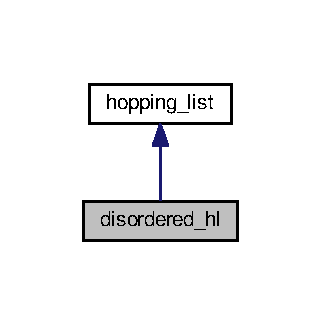
\includegraphics[width=154pt]{structdisordered__hl__inherit__graph}
\end{center}
\end{figure}


Collaboration diagram for disordered\+\_\+hl\+:\nopagebreak
\begin{figure}[H]
\begin{center}
\leavevmode
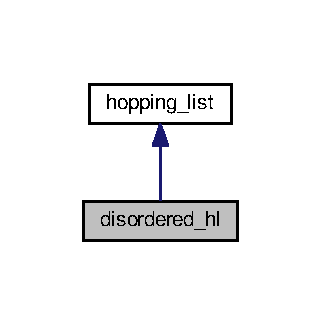
\includegraphics[width=154pt]{structdisordered__hl__coll__graph}
\end{center}
\end{figure}
\subsection*{Additional Inherited Members}


The documentation for this struct was generated from the following file\+:\begin{DoxyCompactItemize}
\item 
/data/jgarcia/codes/linqt/utilities/wannier2sparse/include/disordered\+\_\+hopping\+\_\+list.\+hpp\end{DoxyCompactItemize}

\hypertarget{classhopping__kind}{}\section{hopping\+\_\+kind Class Reference}
\label{classhopping__kind}\index{hopping\+\_\+kind@{hopping\+\_\+kind}}
\subsection*{Public Types}
\begin{DoxyCompactItemize}
\item 
typedef complex$<$ double $>$ {\bfseries value\+\_\+t}\hypertarget{classhopping__kind_ade6db5b12bf7dad2bd590283e955be31}{}\label{classhopping__kind_ade6db5b12bf7dad2bd590283e955be31}

\item 
typedef default\+\_\+random\+\_\+engine {\bfseries random\+\_\+generator}\hypertarget{classhopping__kind_a08b2df934be57ad9fa7aee520bdd3341}{}\label{classhopping__kind_a08b2df934be57ad9fa7aee520bdd3341}

\end{DoxyCompactItemize}
\subsection*{Public Member Functions}
\begin{DoxyCompactItemize}
\item 
{\bfseries hopping\+\_\+kind} (value\+\_\+t \+\_\+hop)\hypertarget{classhopping__kind_ab16319e7f52d80a89ae2e0a46051259a}{}\label{classhopping__kind_ab16319e7f52d80a89ae2e0a46051259a}

\item 
value\+\_\+t {\bfseries operator()} ()\hypertarget{classhopping__kind_a7b895a4fe5b6b57c163bf11d46e182af}{}\label{classhopping__kind_a7b895a4fe5b6b57c163bf11d46e182af}

\item 
\hyperlink{classhopping__kind}{hopping\+\_\+kind} {\bfseries Concentration} (double concentration)\hypertarget{classhopping__kind_a9e53733315f2d6d98771e46e6e7a1152}{}\label{classhopping__kind_a9e53733315f2d6d98771e46e6e7a1152}

\item 
\hyperlink{classhopping__kind}{hopping\+\_\+kind} {\bfseries Distribution\+Type} (string \&distribution, const value\+\_\+t \&min\+\_\+val, const value\+\_\+t \&max\+\_\+val)\hypertarget{classhopping__kind_a799eb93b41c08eaffdb776b2d76e3925}{}\label{classhopping__kind_a799eb93b41c08eaffdb776b2d76e3925}

\item 
void {\bfseries Rescale} (const value\+\_\+t \&scalfact)\hypertarget{classhopping__kind_a95dd8a4b29d2706bb4b4abe41aef1a59}{}\label{classhopping__kind_a95dd8a4b29d2706bb4b4abe41aef1a59}

\item 
bool {\bfseries is\+\_\+constant} () const \hypertarget{classhopping__kind_a78367703ba07a91fc340ae19d5a9e69d}{}\label{classhopping__kind_a78367703ba07a91fc340ae19d5a9e69d}

\end{DoxyCompactItemize}


The documentation for this class was generated from the following file\+:\begin{DoxyCompactItemize}
\item 
/data/jgarcia/codes/linqt/utilities/wannier2sparse/include/hopping\+\_\+kind.\+hpp\end{DoxyCompactItemize}

\hypertarget{classhopping__list}{}\section{hopping\+\_\+list Class Reference}
\label{classhopping__list}\index{hopping\+\_\+list@{hopping\+\_\+list}}


{\ttfamily \#include $<$hopping\+\_\+list.\+hpp$>$}



Inheritance diagram for hopping\+\_\+list\+:\nopagebreak
\begin{figure}[H]
\begin{center}
\leavevmode
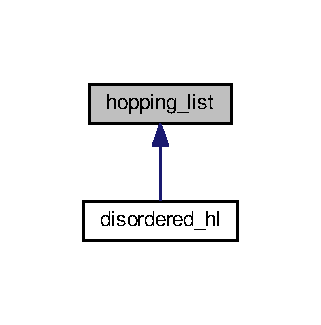
\includegraphics[width=154pt]{classhopping__list__inherit__graph}
\end{center}
\end{figure}
\subsection*{Public Types}
\begin{DoxyCompactItemize}
\item 
typedef \hyperlink{classhopping__kind}{hopping\+\_\+kind} {\bfseries hopkind\+\_\+t}\hypertarget{classhopping__list_add5e4657724bc845ddac46d72a595feb}{}\label{classhopping__list_add5e4657724bc845ddac46d72a595feb}

\item 
typedef hopkind\+\_\+t\+::value\+\_\+t {\bfseries value\+\_\+t}\hypertarget{classhopping__list_af135e2651c597b6aab5ed797898fb974}{}\label{classhopping__list_af135e2651c597b6aab5ed797898fb974}

\item 
typedef array$<$ int, 2 $>$ {\bfseries edge\+\_\+t}\hypertarget{classhopping__list_abc3b58fecac198fd51d62c72ce97dcc5}{}\label{classhopping__list_abc3b58fecac198fd51d62c72ce97dcc5}

\item 
typedef array$<$ int, 3 $>$ {\bfseries cell\+I\+D\+\_\+t}\hypertarget{classhopping__list_a2a22c580c766f39bf5cc017b997e45a0}{}\label{classhopping__list_a2a22c580c766f39bf5cc017b997e45a0}

\item 
typedef tuple$<$ cell\+I\+D\+\_\+t, \hyperlink{classhopping__kind}{hopkind\+\_\+t}, edge\+\_\+t $>$ {\bfseries hopping\+\_\+t}\hypertarget{classhopping__list_a9ea94139b2c4de15b44d8b9701ef2983}{}\label{classhopping__list_a9ea94139b2c4de15b44d8b9701ef2983}

\end{DoxyCompactItemize}
\subsection*{Public Member Functions}
\begin{DoxyCompactItemize}
\item 
\hyperlink{classhopping__list_afaed7dcbb41d5574b29a1bdf10302539}{hopping\+\_\+list} ()
\item 
int \hyperlink{classhopping__list_ae128c276220b0da9b2fcd92632ade569}{Wannier\+Basis\+Size} () const 
\item 
void \hyperlink{classhopping__list_a1b279de0f9c4bc23483245007bb43dd0}{Set\+Wannier\+Basis\+Size} (const int num\+\_\+wann)
\item 
cell\+I\+D\+\_\+t \hyperlink{classhopping__list_afaac6d4d4ff81f11856b62a05b0cf7a2}{Bounds} ()
\item 
void \hyperlink{classhopping__list_abb88b998a8960ca5a9a1c9a83dc316e6}{Set\+Bounds} (const cell\+I\+D\+\_\+t \&cell\+Sizes)
\item 
int \hyperlink{classhopping__list_a1d2ed0ea1881423174565d48fdd8eb7e}{cell\+I\+D\+\_\+index} (const cell\+I\+D\+\_\+t cidx)
\item 
void \hyperlink{classhopping__list_ac6306e64f621457e02eebe91597da8ba}{Add\+Hopping} (const cell\+I\+D\+\_\+t \&\+\_\+cell\+ID, const value\+\_\+t \&\+\_\+value, const edge\+\_\+t \&\+\_\+edge)
\item 
void \hyperlink{classhopping__list_a6f368e8d15bfe657eb4878837be01941}{Add\+Hopping} (const cell\+I\+D\+\_\+t \&\+\_\+cell\+ID, const \hyperlink{classhopping__kind}{hopping\+\_\+kind} \&\+\_\+hop, const edge\+\_\+t \&\+\_\+edge)
\item 
void \hyperlink{classhopping__list_a6eab8d8939b7c5343688831cb842bb92}{Add\+Hopping} (const string \&tag, const hopping\+\_\+t \&hop)
\item 
void \hyperlink{classhopping__list_ac23a0793888fd149e156d15d984bb0ce}{Scale\+Hopping} (cell\+I\+D\+\_\+t \+\_\+cell\+ID, value\+\_\+t \+\_\+value, edge\+\_\+t \+\_\+edge)
\item 
string \hyperlink{classhopping__list_a975de806f3712c94cf28687951a5d0c2}{get\+\_\+tag} (const hopping\+\_\+list\+::cell\+I\+D\+\_\+t \&cid, const hopping\+\_\+list\+::edge\+\_\+t edge)
\item 
\hyperlink{classhopping__list}{hopping\+\_\+list} \& \hyperlink{classhopping__list_a34db85b21f0ef09211e3d453982bf00b}{add\+\_\+from\+\_\+wannier} (tuple$<$ int, vector$<$ string $>$ $>$ wannier\+\_\+data)
\item 
\hyperlink{classhopping__list}{hopping\+\_\+list} \& \hyperlink{classhopping__list_a519475380fef3fb16f5c3dfced395348}{add\+\_\+random\+\_\+hopping\+\_\+list} (vector$<$ vector$<$ string $>$ $>$ disorder\+\_\+data)
\item 
\hyperlink{classhopping__list}{hopping\+\_\+list} \hyperlink{classhopping__list_ad1c6f8098b37731b07d1c76299f8a999}{wrap\+\_\+in\+\_\+supercell} (const hopping\+\_\+list\+::cell\+I\+D\+\_\+t \&cell\+Dim)
\item 
void \hyperlink{classhopping__list_ae1ac0162da77e318faefd6437ecca62d}{save\+\_\+hopping\+\_\+list\+\_\+as\+\_\+csr} (string output\+\_\+filename)
\item 
bool {\bfseries operator==} (\hyperlink{classhopping__list}{hopping\+\_\+list} \&y)\hypertarget{classhopping__list_a64694bc68e64ec1e7a6a418696948c0e}{}\label{classhopping__list_a64694bc68e64ec1e7a6a418696948c0e}

\end{DoxyCompactItemize}
\subsection*{Public Attributes}
\begin{DoxyCompactItemize}
\item 
multimap$<$ string, hopping\+\_\+t $>$ {\bfseries hoppings}\hypertarget{classhopping__list_a33757f5dc87ae85c7867ea2c56ef9838}{}\label{classhopping__list_a33757f5dc87ae85c7867ea2c56ef9838}

\end{DoxyCompactItemize}


\subsection{Detailed Description}
The \hyperlink{classhopping__list}{hopping\+\_\+list} class handles the hoppings of wannier2sparse. This class parse the hoppings from the input files 

\subsection{Constructor \& Destructor Documentation}
\index{hopping\+\_\+list@{hopping\+\_\+list}!hopping\+\_\+list@{hopping\+\_\+list}}
\index{hopping\+\_\+list@{hopping\+\_\+list}!hopping\+\_\+list@{hopping\+\_\+list}}
\subsubsection[{\texorpdfstring{hopping\+\_\+list()}{hopping_list()}}]{\setlength{\rightskip}{0pt plus 5cm}hopping\+\_\+list\+::hopping\+\_\+list (
\begin{DoxyParamCaption}
{}
\end{DoxyParamCaption}
)\hspace{0.3cm}{\ttfamily [inline]}}\hypertarget{classhopping__list_afaed7dcbb41d5574b29a1bdf10302539}{}\label{classhopping__list_afaed7dcbb41d5574b29a1bdf10302539}
Construct hopping list which posses no wannier functions and it is assume to exist on a single cell 

\subsection{Member Function Documentation}
\index{hopping\+\_\+list@{hopping\+\_\+list}!add\+\_\+from\+\_\+wannier@{add\+\_\+from\+\_\+wannier}}
\index{add\+\_\+from\+\_\+wannier@{add\+\_\+from\+\_\+wannier}!hopping\+\_\+list@{hopping\+\_\+list}}
\subsubsection[{\texorpdfstring{add\+\_\+from\+\_\+wannier(tuple$<$ int, vector$<$ string $>$ $>$ wannier\+\_\+data)}{add_from_wannier(tuple< int, vector< string > > wannier_data)}}]{\setlength{\rightskip}{0pt plus 5cm}{\bf hopping\+\_\+list} \& hopping\+\_\+list\+::add\+\_\+from\+\_\+wannier (
\begin{DoxyParamCaption}
\item[{tuple$<$ int, vector$<$ string $>$ $>$}]{wannier\+\_\+data}
\end{DoxyParamCaption}
)}\hypertarget{classhopping__list_a34db85b21f0ef09211e3d453982bf00b}{}\label{classhopping__list_a34db85b21f0ef09211e3d453982bf00b}
Parse the hoppings from a \+\_\+hr.\+dat file 
\begin{DoxyParams}[1]{Parameters}
\mbox{\tt in}  & {\em Wannier\+Data} & Tuple containing the number of wannier basis, and strings read from the wannier\+\_\+hr.\+dat file containing the wannier operator. \\
\hline
\end{DoxyParams}
\begin{DoxyReturn}{Returns}
\hyperlink{classhopping__list}{hopping\+\_\+list} Returns a pointer to a modified \hyperlink{classhopping__list}{hopping\+\_\+list} containing this hoppings. 
\end{DoxyReturn}
\index{hopping\+\_\+list@{hopping\+\_\+list}!add\+\_\+random\+\_\+hopping\+\_\+list@{add\+\_\+random\+\_\+hopping\+\_\+list}}
\index{add\+\_\+random\+\_\+hopping\+\_\+list@{add\+\_\+random\+\_\+hopping\+\_\+list}!hopping\+\_\+list@{hopping\+\_\+list}}
\subsubsection[{\texorpdfstring{add\+\_\+random\+\_\+hopping\+\_\+list(vector$<$ vector$<$ string $>$ $>$ disorder\+\_\+data)}{add_random_hopping_list(vector< vector< string > > disorder_data)}}]{\setlength{\rightskip}{0pt plus 5cm}{\bf hopping\+\_\+list} \& hopping\+\_\+list\+::add\+\_\+random\+\_\+hopping\+\_\+list (
\begin{DoxyParamCaption}
\item[{vector$<$ vector$<$ string $>$ $>$}]{disorder\+\_\+data}
\end{DoxyParamCaption}
)}\hypertarget{classhopping__list_a519475380fef3fb16f5c3dfced395348}{}\label{classhopping__list_a519475380fef3fb16f5c3dfced395348}
Add a set of hoppings with a random component from a hopping file 
\begin{DoxyParams}[1]{Parameters}
\mbox{\tt in}  & {\em hopping\+\_\+data} & Vector containingstrings read from the wannier\+\_\+hr.\+dat file containing the wannier operator. \\
\hline
\end{DoxyParams}
\begin{DoxyReturn}{Returns}
\hyperlink{classhopping__list}{hopping\+\_\+list} Returns a pointer to a modified \hyperlink{classhopping__list}{hopping\+\_\+list} containing this hoppings. 
\end{DoxyReturn}
\index{hopping\+\_\+list@{hopping\+\_\+list}!Add\+Hopping@{Add\+Hopping}}
\index{Add\+Hopping@{Add\+Hopping}!hopping\+\_\+list@{hopping\+\_\+list}}
\subsubsection[{\texorpdfstring{Add\+Hopping(const cell\+I\+D\+\_\+t \&\+\_\+cell\+I\+D, const value\+\_\+t \&\+\_\+value, const edge\+\_\+t \&\+\_\+edge)}{AddHopping(const cellID_t &_cellID, const value_t &_value, const edge_t &_edge)}}]{\setlength{\rightskip}{0pt plus 5cm}void hopping\+\_\+list\+::\+Add\+Hopping (
\begin{DoxyParamCaption}
\item[{const cell\+I\+D\+\_\+t \&}]{\+\_\+cell\+ID, }
\item[{const value\+\_\+t \&}]{\+\_\+value, }
\item[{const edge\+\_\+t \&}]{\+\_\+edge}
\end{DoxyParamCaption}
)}\hypertarget{classhopping__list_ac6306e64f621457e02eebe91597da8ba}{}\label{classhopping__list_ac6306e64f621457e02eebe91597da8ba}
Add this hopping to the hopping list. If the hopping already exists, add it as a different hopping with the same tag.


\begin{DoxyParams}[1]{Parameters}
\mbox{\tt in}  & {\em cell\+ID} & Destintation cell ID. \\
\hline
\mbox{\tt in}  & {\em value} & Hopping value. \\
\hline
\mbox{\tt in}  & {\em edge} & Initial and final orbital ID. \\
\hline
\end{DoxyParams}
\index{hopping\+\_\+list@{hopping\+\_\+list}!Add\+Hopping@{Add\+Hopping}}
\index{Add\+Hopping@{Add\+Hopping}!hopping\+\_\+list@{hopping\+\_\+list}}
\subsubsection[{\texorpdfstring{Add\+Hopping(const cell\+I\+D\+\_\+t \&\+\_\+cell\+I\+D, const hopping\+\_\+kind \&\+\_\+hop, const edge\+\_\+t \&\+\_\+edge)}{AddHopping(const cellID_t &_cellID, const hopping_kind &_hop, const edge_t &_edge)}}]{\setlength{\rightskip}{0pt plus 5cm}void hopping\+\_\+list\+::\+Add\+Hopping (
\begin{DoxyParamCaption}
\item[{const cell\+I\+D\+\_\+t \&}]{\+\_\+cell\+ID, }
\item[{const {\bf hopping\+\_\+kind} \&}]{\+\_\+hop, }
\item[{const edge\+\_\+t \&}]{\+\_\+edge}
\end{DoxyParamCaption}
)}\hypertarget{classhopping__list_a6f368e8d15bfe657eb4878837be01941}{}\label{classhopping__list_a6f368e8d15bfe657eb4878837be01941}
Add this hopping to the hopping list. If the hopping already exists, add it as a different hopping with the same tag.


\begin{DoxyParams}[1]{Parameters}
\mbox{\tt in}  & {\em cell\+ID} & Destintation cell ID. \\
\hline
\mbox{\tt in}  & {\em value} & Hopping Kind. \\
\hline
\mbox{\tt in}  & {\em edge} & Initial and final orbital ID. \\
\hline
\end{DoxyParams}
\index{hopping\+\_\+list@{hopping\+\_\+list}!Add\+Hopping@{Add\+Hopping}}
\index{Add\+Hopping@{Add\+Hopping}!hopping\+\_\+list@{hopping\+\_\+list}}
\subsubsection[{\texorpdfstring{Add\+Hopping(const string \&tag, const hopping\+\_\+t \&hop)}{AddHopping(const string &tag, const hopping_t &hop)}}]{\setlength{\rightskip}{0pt plus 5cm}void hopping\+\_\+list\+::\+Add\+Hopping (
\begin{DoxyParamCaption}
\item[{const string \&}]{tag, }
\item[{const hopping\+\_\+t \&}]{hop}
\end{DoxyParamCaption}
)}\hypertarget{classhopping__list_a6eab8d8939b7c5343688831cb842bb92}{}\label{classhopping__list_a6eab8d8939b7c5343688831cb842bb92}
Add this hopping to the hopping list. If the hopping already exists, add it as a different hopping with the same tag.


\begin{DoxyParams}[1]{Parameters}
\mbox{\tt in}  & {\em cell\+ID} & Destintation cell ID. \\
\hline
\mbox{\tt in}  & {\em value} & Hopping Kind. \\
\hline
\mbox{\tt in}  & {\em edge} & Initial and final orbital ID. \\
\hline
\end{DoxyParams}
\index{hopping\+\_\+list@{hopping\+\_\+list}!Bounds@{Bounds}}
\index{Bounds@{Bounds}!hopping\+\_\+list@{hopping\+\_\+list}}
\subsubsection[{\texorpdfstring{Bounds()}{Bounds()}}]{\setlength{\rightskip}{0pt plus 5cm}cell\+I\+D\+\_\+t hopping\+\_\+list\+::\+Bounds (
\begin{DoxyParamCaption}
{}
\end{DoxyParamCaption}
)\hspace{0.3cm}{\ttfamily [inline]}}\hypertarget{classhopping__list_afaac6d4d4ff81f11856b62a05b0cf7a2}{}\label{classhopping__list_afaac6d4d4ff81f11856b62a05b0cf7a2}
Return the number of unit cells needed to define the hoppings.

\begin{DoxyReturn}{Returns}
cell\+Sizes A three dimensional array containing the number of unit cells in each spatial direction 
\end{DoxyReturn}
\index{hopping\+\_\+list@{hopping\+\_\+list}!cell\+I\+D\+\_\+index@{cell\+I\+D\+\_\+index}}
\index{cell\+I\+D\+\_\+index@{cell\+I\+D\+\_\+index}!hopping\+\_\+list@{hopping\+\_\+list}}
\subsubsection[{\texorpdfstring{cell\+I\+D\+\_\+index(const cell\+I\+D\+\_\+t cidx)}{cellID_index(const cellID_t cidx)}}]{\setlength{\rightskip}{0pt plus 5cm}int hopping\+\_\+list\+::cell\+I\+D\+\_\+index (
\begin{DoxyParamCaption}
\item[{const cell\+I\+D\+\_\+t}]{cidx}
\end{DoxyParamCaption}
)\hspace{0.3cm}{\ttfamily [inline]}}\hypertarget{classhopping__list_a1d2ed0ea1881423174565d48fdd8eb7e}{}\label{classhopping__list_a1d2ed0ea1881423174565d48fdd8eb7e}
Return the number of unit cells needed to define the hoppings in a given direction. 
\begin{DoxyParams}[1]{Parameters}
\mbox{\tt in}  & {\em dir} & The direction index =0,1,2, where the number of unit cells is required. \\
\hline
\end{DoxyParams}
\begin{DoxyReturn}{Returns}
cell\+Size\mbox{[}dir\mbox{]} Number of unit cells in the dir direction. 
\end{DoxyReturn}
\index{hopping\+\_\+list@{hopping\+\_\+list}!get\+\_\+tag@{get\+\_\+tag}}
\index{get\+\_\+tag@{get\+\_\+tag}!hopping\+\_\+list@{hopping\+\_\+list}}
\subsubsection[{\texorpdfstring{get\+\_\+tag(const hopping\+\_\+list\+::cell\+I\+D\+\_\+t \&cid, const hopping\+\_\+list\+::edge\+\_\+t edge)}{get_tag(const hopping_list::cellID_t &cid, const hopping_list::edge_t edge)}}]{\setlength{\rightskip}{0pt plus 5cm}string hopping\+\_\+list\+::get\+\_\+tag (
\begin{DoxyParamCaption}
\item[{const hopping\+\_\+list\+::cell\+I\+D\+\_\+t \&}]{cid, }
\item[{const hopping\+\_\+list\+::edge\+\_\+t}]{edge}
\end{DoxyParamCaption}
)\hspace{0.3cm}{\ttfamily [inline]}}\hypertarget{classhopping__list_a975de806f3712c94cf28687951a5d0c2}{}\label{classhopping__list_a975de806f3712c94cf28687951a5d0c2}
Return the tag string from a given Destination Cell ID and edge.


\begin{DoxyParams}[1]{Parameters}
\mbox{\tt in}  & {\em cell\+ID} & Destintation cell ID. \\
\hline
\mbox{\tt in}  & {\em edge} & Initial and final orbital ID. \\
\hline
\end{DoxyParams}
\begin{DoxyReturn}{Returns}
Tag String defining the tag of the system. 
\end{DoxyReturn}
\index{hopping\+\_\+list@{hopping\+\_\+list}!save\+\_\+hopping\+\_\+list\+\_\+as\+\_\+csr@{save\+\_\+hopping\+\_\+list\+\_\+as\+\_\+csr}}
\index{save\+\_\+hopping\+\_\+list\+\_\+as\+\_\+csr@{save\+\_\+hopping\+\_\+list\+\_\+as\+\_\+csr}!hopping\+\_\+list@{hopping\+\_\+list}}
\subsubsection[{\texorpdfstring{save\+\_\+hopping\+\_\+list\+\_\+as\+\_\+csr(string output\+\_\+filename)}{save_hopping_list_as_csr(string output_filename)}}]{\setlength{\rightskip}{0pt plus 5cm}void hopping\+\_\+list\+::save\+\_\+hopping\+\_\+list\+\_\+as\+\_\+csr (
\begin{DoxyParamCaption}
\item[{string}]{output\+\_\+filename}
\end{DoxyParamCaption}
)}\hypertarget{classhopping__list_ae1ac0162da77e318faefd6437ecca62d}{}\label{classhopping__list_ae1ac0162da77e318faefd6437ecca62d}
Transform the hopping list into C\+SR sparse matrix format, and save it to a file. 
\begin{DoxyParams}[1]{Parameters}
\mbox{\tt in}  & {\em output\+\_\+filename} & Name of the file which will be used to save the hopping list . \\
\hline
\end{DoxyParams}
\index{hopping\+\_\+list@{hopping\+\_\+list}!Scale\+Hopping@{Scale\+Hopping}}
\index{Scale\+Hopping@{Scale\+Hopping}!hopping\+\_\+list@{hopping\+\_\+list}}
\subsubsection[{\texorpdfstring{Scale\+Hopping(cell\+I\+D\+\_\+t \+\_\+cell\+I\+D, value\+\_\+t \+\_\+value, edge\+\_\+t \+\_\+edge)}{ScaleHopping(cellID_t _cellID, value_t _value, edge_t _edge)}}]{\setlength{\rightskip}{0pt plus 5cm}void hopping\+\_\+list\+::\+Scale\+Hopping (
\begin{DoxyParamCaption}
\item[{cell\+I\+D\+\_\+t}]{\+\_\+cell\+ID, }
\item[{value\+\_\+t}]{\+\_\+value, }
\item[{edge\+\_\+t}]{\+\_\+edge}
\end{DoxyParamCaption}
)}\hypertarget{classhopping__list_ac23a0793888fd149e156d15d984bb0ce}{}\label{classhopping__list_ac23a0793888fd149e156d15d984bb0ce}
Scale the hopping defined by its Destination cell ID and its edge. If it does not exists, nothing happens.


\begin{DoxyParams}[1]{Parameters}
\mbox{\tt in}  & {\em cell\+ID} & Destintation cell ID. \\
\hline
\mbox{\tt in}  & {\em value} & Value used for rescaling the hopping hop(cell\+I\+D,edge). \\
\hline
\mbox{\tt in}  & {\em edge} & Initial and final orbital ID. \\
\hline
\end{DoxyParams}
\index{hopping\+\_\+list@{hopping\+\_\+list}!Set\+Bounds@{Set\+Bounds}}
\index{Set\+Bounds@{Set\+Bounds}!hopping\+\_\+list@{hopping\+\_\+list}}
\subsubsection[{\texorpdfstring{Set\+Bounds(const cell\+I\+D\+\_\+t \&cell\+Sizes)}{SetBounds(const cellID_t &cellSizes)}}]{\setlength{\rightskip}{0pt plus 5cm}void hopping\+\_\+list\+::\+Set\+Bounds (
\begin{DoxyParamCaption}
\item[{const cell\+I\+D\+\_\+t \&}]{cell\+Sizes}
\end{DoxyParamCaption}
)\hspace{0.3cm}{\ttfamily [inline]}}\hypertarget{classhopping__list_abb88b998a8960ca5a9a1c9a83dc316e6}{}\label{classhopping__list_abb88b998a8960ca5a9a1c9a83dc316e6}
Set the number of unit cells needed to define the hoppings.


\begin{DoxyParams}[1]{Parameters}
\mbox{\tt in}  & {\em cell\+Sizes} & A three dimensional array containing the number of unit cells in each spatial direction \\
\hline
\end{DoxyParams}
\index{hopping\+\_\+list@{hopping\+\_\+list}!Set\+Wannier\+Basis\+Size@{Set\+Wannier\+Basis\+Size}}
\index{Set\+Wannier\+Basis\+Size@{Set\+Wannier\+Basis\+Size}!hopping\+\_\+list@{hopping\+\_\+list}}
\subsubsection[{\texorpdfstring{Set\+Wannier\+Basis\+Size(const int num\+\_\+wann)}{SetWannierBasisSize(const int num_wann)}}]{\setlength{\rightskip}{0pt plus 5cm}void hopping\+\_\+list\+::\+Set\+Wannier\+Basis\+Size (
\begin{DoxyParamCaption}
\item[{const int}]{num\+\_\+wann}
\end{DoxyParamCaption}
)\hspace{0.3cm}{\ttfamily [inline]}}\hypertarget{classhopping__list_a1b279de0f9c4bc23483245007bb43dd0}{}\label{classhopping__list_a1b279de0f9c4bc23483245007bb43dd0}
Return Set the size of the Wannier Basis number.


\begin{DoxyParams}[1]{Parameters}
\mbox{\tt in}  & {\em num\+\_\+wann} & Wannier Basis Size. \\
\hline
\end{DoxyParams}
\index{hopping\+\_\+list@{hopping\+\_\+list}!Wannier\+Basis\+Size@{Wannier\+Basis\+Size}}
\index{Wannier\+Basis\+Size@{Wannier\+Basis\+Size}!hopping\+\_\+list@{hopping\+\_\+list}}
\subsubsection[{\texorpdfstring{Wannier\+Basis\+Size() const }{WannierBasisSize() const }}]{\setlength{\rightskip}{0pt plus 5cm}int hopping\+\_\+list\+::\+Wannier\+Basis\+Size (
\begin{DoxyParamCaption}
{}
\end{DoxyParamCaption}
) const\hspace{0.3cm}{\ttfamily [inline]}}\hypertarget{classhopping__list_ae128c276220b0da9b2fcd92632ade569}{}\label{classhopping__list_ae128c276220b0da9b2fcd92632ade569}
Return the Size of the Wannier Basis number.

\begin{DoxyReturn}{Returns}
real component 
\end{DoxyReturn}
\index{hopping\+\_\+list@{hopping\+\_\+list}!wrap\+\_\+in\+\_\+supercell@{wrap\+\_\+in\+\_\+supercell}}
\index{wrap\+\_\+in\+\_\+supercell@{wrap\+\_\+in\+\_\+supercell}!hopping\+\_\+list@{hopping\+\_\+list}}
\subsubsection[{\texorpdfstring{wrap\+\_\+in\+\_\+supercell(const hopping\+\_\+list\+::cell\+I\+D\+\_\+t \&cell\+Dim)}{wrap_in_supercell(const hopping_list::cellID_t &cellDim)}}]{\setlength{\rightskip}{0pt plus 5cm}{\bf hopping\+\_\+list} hopping\+\_\+list\+::wrap\+\_\+in\+\_\+supercell (
\begin{DoxyParamCaption}
\item[{const hopping\+\_\+list\+::cell\+I\+D\+\_\+t \&}]{cell\+Dim}
\end{DoxyParamCaption}
)}\hypertarget{classhopping__list_ad1c6f8098b37731b07d1c76299f8a999}{}\label{classhopping__list_ad1c6f8098b37731b07d1c76299f8a999}
Embedded the system into a supercell. This procedure changes the destination cell of all hoppings, adding them when needed. It also changes the initial and final orbital ID in order to accomodate the inner atoms of the new supercell. 
\begin{DoxyParams}[1]{Parameters}
\mbox{\tt in}  & {\em cell\+Dim} & New supercell over which the hoppings are defined. \\
\hline
\end{DoxyParams}
\begin{DoxyReturn}{Returns}
\hyperlink{classhopping__list}{hopping\+\_\+list} Returns a pointer to a modified \hyperlink{classhopping__list}{hopping\+\_\+list} defined over a new unit cells. 
\end{DoxyReturn}


The documentation for this class was generated from the following files\+:\begin{DoxyCompactItemize}
\item 
/data/jgarcia/codes/linqt/utilities/wannier2sparse/include/hopping\+\_\+list.\+hpp\item 
/data/jgarcia/codes/linqt/utilities/wannier2sparse/src/hopping\+\_\+list.\+cpp\end{DoxyCompactItemize}

\hypertarget{classchebyshev_1_1_moments}{}\section{chebyshev\+:\+:Moments Class Reference}
\label{classchebyshev_1_1_moments}\index{chebyshev\+::\+Moments@{chebyshev\+::\+Moments}}


Inheritance diagram for chebyshev\+:\+:Moments\+:\nopagebreak
\begin{figure}[H]
\begin{center}
\leavevmode
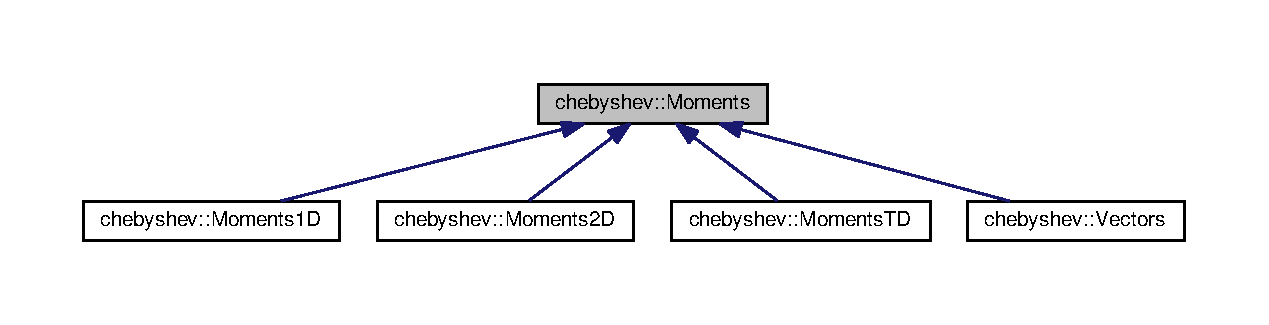
\includegraphics[width=350pt]{classchebyshev_1_1_moments__inherit__graph}
\end{center}
\end{figure}
\subsection*{Public Types}
\begin{DoxyCompactItemize}
\item 
typedef std\+::complex$<$ double $>$ {\bfseries value\+\_\+t}\hypertarget{classchebyshev_1_1_moments_a23e4a9b2eebf82d5fc6c849327cbd3d8}{}\label{classchebyshev_1_1_moments_a23e4a9b2eebf82d5fc6c849327cbd3d8}

\item 
typedef std\+::vector$<$ value\+\_\+t $>$ {\bfseries vector\+\_\+t}\hypertarget{classchebyshev_1_1_moments_a711a270332e05270a18a6a186ce00657}{}\label{classchebyshev_1_1_moments_a711a270332e05270a18a6a186ce00657}

\end{DoxyCompactItemize}
\subsection*{Public Member Functions}
\begin{DoxyCompactItemize}
\item 
size\+\_\+t {\bfseries System\+Size} () const \hypertarget{classchebyshev_1_1_moments_a643ac4793661d07fb5468ccdbda4d274}{}\label{classchebyshev_1_1_moments_a643ac4793661d07fb5468ccdbda4d274}

\item 
string {\bfseries System\+Label} () const \hypertarget{classchebyshev_1_1_moments_aeae3162cd5f930affcc5b282c0ed2929}{}\label{classchebyshev_1_1_moments_aeae3162cd5f930affcc5b282c0ed2929}

\item 
double {\bfseries Band\+Width} () const \hypertarget{classchebyshev_1_1_moments_a7667fa18bec7c59417e558963fb0e3fd}{}\label{classchebyshev_1_1_moments_a7667fa18bec7c59417e558963fb0e3fd}

\item 
double {\bfseries Half\+Width} () const \hypertarget{classchebyshev_1_1_moments_abad9d579ade5250ca3aa29d643147a73}{}\label{classchebyshev_1_1_moments_abad9d579ade5250ca3aa29d643147a73}

\item 
double {\bfseries Band\+Center} () const \hypertarget{classchebyshev_1_1_moments_a79a6dc22ec1d546fda69aba33febcc2c}{}\label{classchebyshev_1_1_moments_a79a6dc22ec1d546fda69aba33febcc2c}

\item 
double {\bfseries Scale\+Factor} () const \hypertarget{classchebyshev_1_1_moments_affb049e07ebc8fe43d6ec2cde0771338}{}\label{classchebyshev_1_1_moments_affb049e07ebc8fe43d6ec2cde0771338}

\item 
double {\bfseries Shift\+Factor} () const \hypertarget{classchebyshev_1_1_moments_a29949dd338081832678a203a0c87ee82}{}\label{classchebyshev_1_1_moments_a29949dd338081832678a203a0c87ee82}

\item 
vector\+\_\+t \& {\bfseries Moment\+Vector} ()\hypertarget{classchebyshev_1_1_moments_aa26cda360676f86281c31ccb2340bd34}{}\label{classchebyshev_1_1_moments_aa26cda360676f86281c31ccb2340bd34}

\item 
value\+\_\+t \& {\bfseries Moment\+Vector} (const int i)\hypertarget{classchebyshev_1_1_moments_aa47e7c74c396d478940ef5dcf3d5e6ed}{}\label{classchebyshev_1_1_moments_aa47e7c74c396d478940ef5dcf3d5e6ed}

\item 
Moments\+::vector\+\_\+t \& {\bfseries Chebyshev0} ()\hypertarget{classchebyshev_1_1_moments_a8634f3562b8c6544397052413d74ecec}{}\label{classchebyshev_1_1_moments_a8634f3562b8c6544397052413d74ecec}

\item 
Moments\+::vector\+\_\+t \& {\bfseries Chebyshev1} ()\hypertarget{classchebyshev_1_1_moments_ab8b932b90a33e13756cadab8c448474b}{}\label{classchebyshev_1_1_moments_ab8b932b90a33e13756cadab8c448474b}

\item 
\hyperlink{class_sparse_matrix_type}{Sparse\+Matrix\+Type} \& {\bfseries Hamiltonian} ()\hypertarget{classchebyshev_1_1_moments_a0deae44c3529c12e14954708f7f5c712}{}\label{classchebyshev_1_1_moments_a0deae44c3529c12e14954708f7f5c712}

\item 
void {\bfseries Set\+Hamiltonian} (\hyperlink{class_sparse_matrix_type}{Sparse\+Matrix\+Type} \&N\+H\+AM)\hypertarget{classchebyshev_1_1_moments_aed05965de8ad9b2dfa4a6c459284ec09}{}\label{classchebyshev_1_1_moments_aed05965de8ad9b2dfa4a6c459284ec09}

\item 
void {\bfseries System\+Size} (const int dim)\hypertarget{classchebyshev_1_1_moments_a27f760f321dea8f7deaee3bd860ae1b9}{}\label{classchebyshev_1_1_moments_a27f760f321dea8f7deaee3bd860ae1b9}

\item 
void {\bfseries System\+Label} (string label)\hypertarget{classchebyshev_1_1_moments_af0e626b9f966c5fd817cbb4ed20b86fb}{}\label{classchebyshev_1_1_moments_af0e626b9f966c5fd817cbb4ed20b86fb}

\item 
void {\bfseries Band\+Width} (const double x)\hypertarget{classchebyshev_1_1_moments_a2537cf25e77630a6f791bfac3eefe433}{}\label{classchebyshev_1_1_moments_a2537cf25e77630a6f791bfac3eefe433}

\item 
void {\bfseries Band\+Center} (const double x)\hypertarget{classchebyshev_1_1_moments_adf3725c46548cb60a20d4164ee20845d}{}\label{classchebyshev_1_1_moments_adf3725c46548cb60a20d4164ee20845d}

\item 
void {\bfseries Moment\+Vector} (const vector\+\_\+t \+\_\+mu)\hypertarget{classchebyshev_1_1_moments_a2f91986d82de1f85e5fc252440749872}{}\label{classchebyshev_1_1_moments_a2f91986d82de1f85e5fc252440749872}

\item 
void {\bfseries Set\+Init\+Vectors} (\hyperlink{class_sparse_matrix_type}{Sparse\+Matrix\+Type} \&N\+H\+AM, \hyperlink{class_sparse_matrix_type}{Sparse\+Matrix\+Type} \&OP, const vector\+\_\+t \&T0)\hypertarget{classchebyshev_1_1_moments_a1edb5a95fc3c55790a1c42dcc0c9d6d8}{}\label{classchebyshev_1_1_moments_a1edb5a95fc3c55790a1c42dcc0c9d6d8}

\item 
void {\bfseries Set\+Init\+Vectors} (const vector\+\_\+t \&T0)\hypertarget{classchebyshev_1_1_moments_a50109c2eb34b8b48fa84259e061b557f}{}\label{classchebyshev_1_1_moments_a50109c2eb34b8b48fa84259e061b557f}

\item 
void {\bfseries Set\+Init\+Vectors} (\hyperlink{class_sparse_matrix_type}{Sparse\+Matrix\+Type} \&OP, const vector\+\_\+t \&T0)\hypertarget{classchebyshev_1_1_moments_a41341eff2a0545d3c742ff4518438a03}{}\label{classchebyshev_1_1_moments_a41341eff2a0545d3c742ff4518438a03}

\item 
double {\bfseries Rescale2\+Chebyshev\+Domain} (const double energ)\hypertarget{classchebyshev_1_1_moments_a113588b1702443cf9242f29f557e3d24}{}\label{classchebyshev_1_1_moments_a113588b1702443cf9242f29f557e3d24}

\item 
int {\bfseries Iterate} (\hyperlink{class_sparse_matrix_type}{Sparse\+Matrix\+Type} \&N\+H\+AM)\hypertarget{classchebyshev_1_1_moments_ac5e8717267207fe9a2ef3477a417cdf3}{}\label{classchebyshev_1_1_moments_ac5e8717267207fe9a2ef3477a417cdf3}

\item 
int {\bfseries Iterate} ()\hypertarget{classchebyshev_1_1_moments_a22a6d744e419f7e6311f52ef3bccfde8}{}\label{classchebyshev_1_1_moments_a22a6d744e419f7e6311f52ef3bccfde8}

\item 
int {\bfseries Jackson\+Kernel\+Mom\+Cut\+Off} (const double broad)\hypertarget{classchebyshev_1_1_moments_ab06aa806c3ffdb165ee6a4722c76b03d}{}\label{classchebyshev_1_1_moments_ab06aa806c3ffdb165ee6a4722c76b03d}

\item 
double {\bfseries Jackson\+Kernel} (const double m, const double Mom)\hypertarget{classchebyshev_1_1_moments_a3c5b8faa133bb4a3b8dc2172812ae483}{}\label{classchebyshev_1_1_moments_a3c5b8faa133bb4a3b8dc2172812ae483}

\item 
int {\bfseries Rescale2\+Chebyshev\+Domain} (\hyperlink{class_sparse_matrix_type}{Sparse\+Matrix\+Type} \&H)\hypertarget{classchebyshev_1_1_moments_adf94ad58234e7cfb3a19eb5ce22fda95}{}\label{classchebyshev_1_1_moments_adf94ad58234e7cfb3a19eb5ce22fda95}

\end{DoxyCompactItemize}


The documentation for this class was generated from the following files\+:\begin{DoxyCompactItemize}
\item 
/data/jgarcia/codes/linqt/include/chebyshev\+\_\+moments.\+hpp\item 
/data/jgarcia/codes/linqt/src/chebyshev\+\_\+moments.\+cpp\end{DoxyCompactItemize}

\hypertarget{classchebyshev_1_1_moments1_d}{}\section{chebyshev\+:\+:Moments1D Class Reference}
\label{classchebyshev_1_1_moments1_d}\index{chebyshev\+::\+Moments1D@{chebyshev\+::\+Moments1D}}


Inheritance diagram for chebyshev\+:\+:Moments1D\+:\nopagebreak
\begin{figure}[H]
\begin{center}
\leavevmode
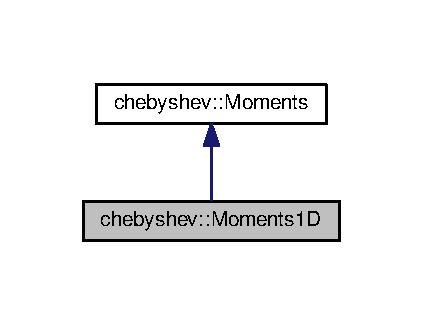
\includegraphics[width=203pt]{classchebyshev_1_1_moments1_d__inherit__graph}
\end{center}
\end{figure}


Collaboration diagram for chebyshev\+:\+:Moments1D\+:\nopagebreak
\begin{figure}[H]
\begin{center}
\leavevmode
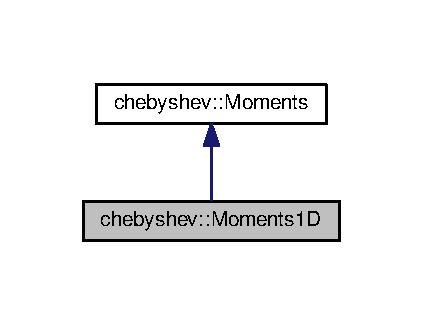
\includegraphics[width=203pt]{classchebyshev_1_1_moments1_d__coll__graph}
\end{center}
\end{figure}
\subsection*{Public Member Functions}
\begin{DoxyCompactItemize}
\item 
{\bfseries Moments1D} (const size\+\_\+t m0)\hypertarget{classchebyshev_1_1_moments1_d_a921572420e08c2746ed6ec7ed409e059}{}\label{classchebyshev_1_1_moments1_d_a921572420e08c2746ed6ec7ed409e059}

\item 
size\+\_\+t {\bfseries Moment\+Number} () const \hypertarget{classchebyshev_1_1_moments1_d_a75667f392f26c85efc222d2ce932d2ee}{}\label{classchebyshev_1_1_moments1_d_a75667f392f26c85efc222d2ce932d2ee}

\item 
size\+\_\+t {\bfseries Highest\+Moment\+Number} () const \hypertarget{classchebyshev_1_1_moments1_d_abbba059822f9998e4d75c04398d4abac}{}\label{classchebyshev_1_1_moments1_d_abbba059822f9998e4d75c04398d4abac}

\item 
Moments\+::value\+\_\+t \& {\bfseries operator()} (const size\+\_\+t m0)\hypertarget{classchebyshev_1_1_moments1_d_a2bfb6aa6b14a637eaa6acf877cf75fb2}{}\label{classchebyshev_1_1_moments1_d_a2bfb6aa6b14a637eaa6acf877cf75fb2}

\item 
void {\bfseries Print} ()\hypertarget{classchebyshev_1_1_moments1_d_abb8de7793a9246acb6830068415353d8}{}\label{classchebyshev_1_1_moments1_d_abb8de7793a9246acb6830068415353d8}

\end{DoxyCompactItemize}
\subsection*{Additional Inherited Members}


The documentation for this class was generated from the following files\+:\begin{DoxyCompactItemize}
\item 
/data/jgarcia/codes/linqt/include/chebyshev\+\_\+moments.\+hpp\item 
/data/jgarcia/codes/linqt/src/chebyshev\+\_\+moments1\+D.\+cpp\end{DoxyCompactItemize}

\hypertarget{classchebyshev_1_1_moments2_d}{}\section{chebyshev\+:\+:Moments2D Class Reference}
\label{classchebyshev_1_1_moments2_d}\index{chebyshev\+::\+Moments2D@{chebyshev\+::\+Moments2D}}


Inheritance diagram for chebyshev\+:\+:Moments2D\+:\nopagebreak
\begin{figure}[H]
\begin{center}
\leavevmode
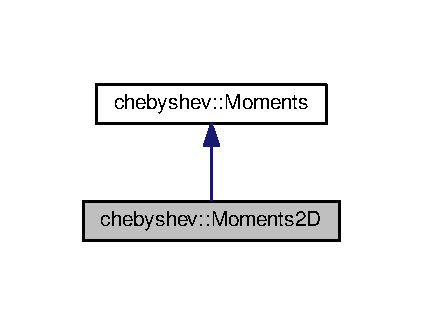
\includegraphics[width=203pt]{classchebyshev_1_1_moments2_d__inherit__graph}
\end{center}
\end{figure}


Collaboration diagram for chebyshev\+:\+:Moments2D\+:\nopagebreak
\begin{figure}[H]
\begin{center}
\leavevmode
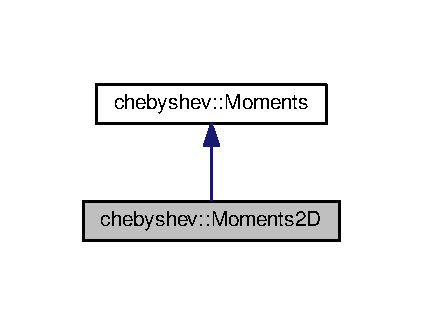
\includegraphics[width=203pt]{classchebyshev_1_1_moments2_d__coll__graph}
\end{center}
\end{figure}
\subsection*{Public Member Functions}
\begin{DoxyCompactItemize}
\item 
{\bfseries Moments2D} (const size\+\_\+t m0, const size\+\_\+t m1)\hypertarget{classchebyshev_1_1_moments2_d_af0b8f711109555572b8d817bef39bbae}{}\label{classchebyshev_1_1_moments2_d_af0b8f711109555572b8d817bef39bbae}

\item 
{\bfseries Moments2D} (std\+::string momfilename)\hypertarget{classchebyshev_1_1_moments2_d_adab0cd1f735cbb3f261c44d7d43b58e5}{}\label{classchebyshev_1_1_moments2_d_adab0cd1f735cbb3f261c44d7d43b58e5}

\item 
array$<$ int, 2 $>$ {\bfseries Moment\+Number} () const \hypertarget{classchebyshev_1_1_moments2_d_a3bf7894afbe847204c61e08b9aa43cde}{}\label{classchebyshev_1_1_moments2_d_a3bf7894afbe847204c61e08b9aa43cde}

\item 
int {\bfseries Highest\+Moment\+Number} (const int i) const \hypertarget{classchebyshev_1_1_moments2_d_a65168ecb2bb52a5bd38b96e1a4df921a}{}\label{classchebyshev_1_1_moments2_d_a65168ecb2bb52a5bd38b96e1a4df921a}

\item 
int {\bfseries Highest\+Moment\+Number} () const \hypertarget{classchebyshev_1_1_moments2_d_ada8a445140a16b5386faa0516a90b6a7}{}\label{classchebyshev_1_1_moments2_d_ada8a445140a16b5386faa0516a90b6a7}

\item 
void {\bfseries Moment\+Number} (const int mom0, const int mom1)\hypertarget{classchebyshev_1_1_moments2_d_af14d8beef67d68836fb6740f44b3597a}{}\label{classchebyshev_1_1_moments2_d_af14d8beef67d68836fb6740f44b3597a}

\item 
Moments\+::value\+\_\+t \& {\bfseries operator()} (const int m0, const int m1)\hypertarget{classchebyshev_1_1_moments2_d_ac762b2cd08185994af2ad805f5b49691}{}\label{classchebyshev_1_1_moments2_d_ac762b2cd08185994af2ad805f5b49691}

\item 
void {\bfseries Apply\+Jackson\+Kernel} (const double b0, const double b1)\hypertarget{classchebyshev_1_1_moments2_d_ad83287368165d03f619b8a7578623b43}{}\label{classchebyshev_1_1_moments2_d_ad83287368165d03f619b8a7578623b43}

\item 
void {\bfseries save\+In} (std\+::string filename)\hypertarget{classchebyshev_1_1_moments2_d_a27dfe3c9ac5e9477fccc1c1fcc3343cf}{}\label{classchebyshev_1_1_moments2_d_a27dfe3c9ac5e9477fccc1c1fcc3343cf}

\item 
void {\bfseries Print} ()\hypertarget{classchebyshev_1_1_moments2_d_a7ace12d910b2fe332192f88fc0785a7c}{}\label{classchebyshev_1_1_moments2_d_a7ace12d910b2fe332192f88fc0785a7c}

\end{DoxyCompactItemize}
\subsection*{Additional Inherited Members}


The documentation for this class was generated from the following files\+:\begin{DoxyCompactItemize}
\item 
/data/jgarcia/codes/linqt/include/chebyshev\+\_\+moments.\+hpp\item 
/data/jgarcia/codes/linqt/src/chebyshev\+\_\+moments2\+D.\+cpp\end{DoxyCompactItemize}

\hypertarget{classchebyshev_1_1_moments_t_d}{}\section{chebyshev\+:\+:Moments\+TD Class Reference}
\label{classchebyshev_1_1_moments_t_d}\index{chebyshev\+::\+Moments\+TD@{chebyshev\+::\+Moments\+TD}}


Inheritance diagram for chebyshev\+:\+:Moments\+TD\+:\nopagebreak
\begin{figure}[H]
\begin{center}
\leavevmode
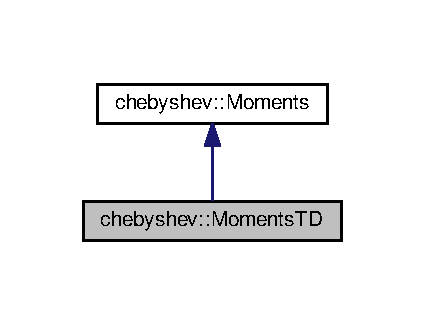
\includegraphics[width=204pt]{classchebyshev_1_1_moments_t_d__inherit__graph}
\end{center}
\end{figure}


Collaboration diagram for chebyshev\+:\+:Moments\+TD\+:\nopagebreak
\begin{figure}[H]
\begin{center}
\leavevmode
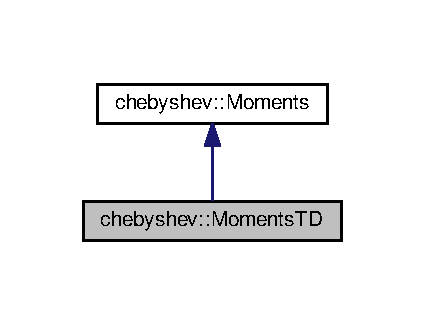
\includegraphics[width=204pt]{classchebyshev_1_1_moments_t_d__coll__graph}
\end{center}
\end{figure}
\subsection*{Public Member Functions}
\begin{DoxyCompactItemize}
\item 
{\bfseries Moments\+TD} (const size\+\_\+t m, const size\+\_\+t n)\hypertarget{classchebyshev_1_1_moments_t_d_acdba269d058b70857247352aa3b47e33}{}\label{classchebyshev_1_1_moments_t_d_acdba269d058b70857247352aa3b47e33}

\item 
{\bfseries Moments\+TD} (std\+::string momfilename)\hypertarget{classchebyshev_1_1_moments_t_d_a9ac2ddc9460bed6c639af179f732c65c}{}\label{classchebyshev_1_1_moments_t_d_a9ac2ddc9460bed6c639af179f732c65c}

\item 
size\+\_\+t {\bfseries Moment\+Number} () const \hypertarget{classchebyshev_1_1_moments_t_d_a3a0b989f9e8f5133ab8a31a67a8838a7}{}\label{classchebyshev_1_1_moments_t_d_a3a0b989f9e8f5133ab8a31a67a8838a7}

\item 
size\+\_\+t {\bfseries Highest\+Moment\+Number} () const \hypertarget{classchebyshev_1_1_moments_t_d_a155e40d181a841fa0e74fbd937be8a1d}{}\label{classchebyshev_1_1_moments_t_d_a155e40d181a841fa0e74fbd937be8a1d}

\item 
size\+\_\+t {\bfseries Current\+Time\+Step} () const \hypertarget{classchebyshev_1_1_moments_t_d_a50fc1e96dd08b5747b33545b36c0be09}{}\label{classchebyshev_1_1_moments_t_d_a50fc1e96dd08b5747b33545b36c0be09}

\item 
size\+\_\+t {\bfseries Max\+Time\+Step} () const \hypertarget{classchebyshev_1_1_moments_t_d_acec2e83ed37f21c275cba99c407660c5}{}\label{classchebyshev_1_1_moments_t_d_acec2e83ed37f21c275cba99c407660c5}

\item 
double {\bfseries Time\+Diff} () const \hypertarget{classchebyshev_1_1_moments_t_d_a03c08c0440b106919f85da1b67406626}{}\label{classchebyshev_1_1_moments_t_d_a03c08c0440b106919f85da1b67406626}

\item 
double {\bfseries Chebyshev\+Freq} () const \hypertarget{classchebyshev_1_1_moments_t_d_a64c512d40aad4baa6eac98f75d684272}{}\label{classchebyshev_1_1_moments_t_d_a64c512d40aad4baa6eac98f75d684272}

\item 
void {\bfseries Moment\+Number} (const size\+\_\+t mom)\hypertarget{classchebyshev_1_1_moments_t_d_aae4fff392f904dd619efc25ec6277a54}{}\label{classchebyshev_1_1_moments_t_d_aae4fff392f904dd619efc25ec6277a54}

\item 
void {\bfseries Max\+Time\+Step} (const size\+\_\+t max\+Time\+Step)\hypertarget{classchebyshev_1_1_moments_t_d_ac6eae9b87f5a2103c09ac2265222ac09}{}\label{classchebyshev_1_1_moments_t_d_ac6eae9b87f5a2103c09ac2265222ac09}

\item 
void {\bfseries Increase\+Time\+Step} ()\hypertarget{classchebyshev_1_1_moments_t_d_a4d19c846719c7bc576600eb1f0f3f3f5}{}\label{classchebyshev_1_1_moments_t_d_a4d19c846719c7bc576600eb1f0f3f3f5}

\item 
void {\bfseries Time\+Diff} (const double dt)\hypertarget{classchebyshev_1_1_moments_t_d_a9affd36141c4059c717c4a1eef6c7e19}{}\label{classchebyshev_1_1_moments_t_d_a9affd36141c4059c717c4a1eef6c7e19}

\item 
void {\bfseries Chebyshev\+Freq} (const double omega)\hypertarget{classchebyshev_1_1_moments_t_d_a874d2bedb2c1a513a48e900a51ec326e}{}\label{classchebyshev_1_1_moments_t_d_a874d2bedb2c1a513a48e900a51ec326e}

\item 
int {\bfseries Evolve} (vector\+\_\+t \&Phi)\hypertarget{classchebyshev_1_1_moments_t_d_a7ddcaee940fd8714ab29f2feaf27633a}{}\label{classchebyshev_1_1_moments_t_d_a7ddcaee940fd8714ab29f2feaf27633a}

\item 
Moments\+::value\+\_\+t \& {\bfseries operator()} (const size\+\_\+t m, const size\+\_\+t n)\hypertarget{classchebyshev_1_1_moments_t_d_a4ee4f9b5054eb24333d0b0197a0f216b}{}\label{classchebyshev_1_1_moments_t_d_a4ee4f9b5054eb24333d0b0197a0f216b}

\item 
void {\bfseries Apply\+Jackson\+Kernel} (const double broad)\hypertarget{classchebyshev_1_1_moments_t_d_a1a208ca21d6b3215ad22ea57653ee156}{}\label{classchebyshev_1_1_moments_t_d_a1a208ca21d6b3215ad22ea57653ee156}

\item 
void {\bfseries save\+In} (std\+::string filename)\hypertarget{classchebyshev_1_1_moments_t_d_aa0ee4348b1e5d27234d7c5c4125b3cea}{}\label{classchebyshev_1_1_moments_t_d_aa0ee4348b1e5d27234d7c5c4125b3cea}

\item 
void {\bfseries Print} ()\hypertarget{classchebyshev_1_1_moments_t_d_a4439f202d47ede1ddd13ade33442d180}{}\label{classchebyshev_1_1_moments_t_d_a4439f202d47ede1ddd13ade33442d180}

\end{DoxyCompactItemize}
\subsection*{Additional Inherited Members}


The documentation for this class was generated from the following files\+:\begin{DoxyCompactItemize}
\item 
/data/jgarcia/codes/linqt/include/chebyshev\+\_\+moments.\+hpp\item 
/data/jgarcia/codes/linqt/src/chebyshev\+\_\+moments\+T\+D.\+cpp\end{DoxyCompactItemize}

\hypertarget{structoputil_1_1op__matrix}{}\section{oputil\+:\+:op\+\_\+matrix Struct Reference}
\label{structoputil_1_1op__matrix}\index{oputil\+::op\+\_\+matrix@{oputil\+::op\+\_\+matrix}}
\subsection*{Public Types}
\begin{DoxyCompactItemize}
\item 
typedef std\+::complex$<$ double $>$ {\bfseries value\+\_\+t}\hypertarget{structoputil_1_1op__matrix_abab9d77ef16c61a8690416a8da709421}{}\label{structoputil_1_1op__matrix_abab9d77ef16c61a8690416a8da709421}

\end{DoxyCompactItemize}
\subsection*{Public Member Functions}
\begin{DoxyCompactItemize}
\item 
{\bfseries op\+\_\+matrix} (const int dim)\hypertarget{structoputil_1_1op__matrix_a92afbe3ef666e8d462b5a12058d4d34f}{}\label{structoputil_1_1op__matrix_a92afbe3ef666e8d462b5a12058d4d34f}

\item 
value\+\_\+t \& {\bfseries operator()} (const int i, const int j)\hypertarget{structoputil_1_1op__matrix_aa414c60df529f0a79c870de17b1699ff}{}\label{structoputil_1_1op__matrix_aa414c60df529f0a79c870de17b1699ff}

\item 
int {\bfseries size} () const \hypertarget{structoputil_1_1op__matrix_a15e6f331488f276a36606e329a0ab319}{}\label{structoputil_1_1op__matrix_a15e6f331488f276a36606e329a0ab319}

\end{DoxyCompactItemize}
\subsection*{Public Attributes}
\begin{DoxyCompactItemize}
\item 
std\+::vector$<$ std\+::vector$<$ value\+\_\+t $>$ $>$ {\bfseries data}\hypertarget{structoputil_1_1op__matrix_ac518c6275c8a0147c5688c5af57bca6f}{}\label{structoputil_1_1op__matrix_ac518c6275c8a0147c5688c5af57bca6f}

\end{DoxyCompactItemize}


The documentation for this struct was generated from the following file\+:\begin{DoxyCompactItemize}
\item 
/data/jgarcia/codes/linqt/utilities/wannier2sparse/include/operator\+\_\+utils.\+hpp\end{DoxyCompactItemize}

\hypertarget{class_sparse_matrix_builder}{}\section{Sparse\+Matrix\+Builder Class Reference}
\label{class_sparse_matrix_builder}\index{Sparse\+Matrix\+Builder@{Sparse\+Matrix\+Builder}}


Collaboration diagram for Sparse\+Matrix\+Builder\+:\nopagebreak
\begin{figure}[H]
\begin{center}
\leavevmode
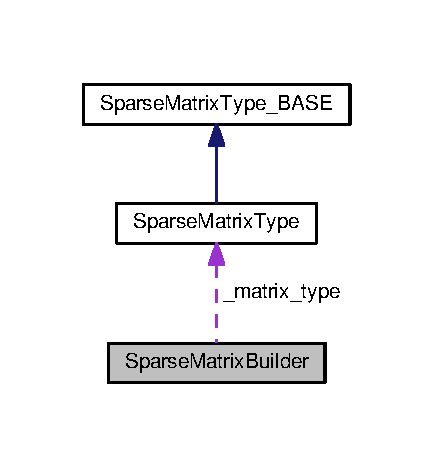
\includegraphics[width=208pt]{class_sparse_matrix_builder__coll__graph}
\end{center}
\end{figure}
\subsection*{Public Member Functions}
\begin{DoxyCompactItemize}
\item 
void {\bfseries set\+Sparse\+Matrix} (\hyperlink{class_sparse_matrix_type}{Sparse\+Matrix\+Type} $\ast$b)\hypertarget{class_sparse_matrix_builder_acff4421ec6c4ef6eac4369f7fb6d8bc3}{}\label{class_sparse_matrix_builder_acff4421ec6c4ef6eac4369f7fb6d8bc3}

\item 
void {\bfseries Build\+O\+P\+From\+C\+S\+R\+File} (const std\+::string input)\hypertarget{class_sparse_matrix_builder_a67bd43b1c8589a74e8fc4ce5a70833cb}{}\label{class_sparse_matrix_builder_a67bd43b1c8589a74e8fc4ce5a70833cb}

\end{DoxyCompactItemize}
\subsection*{Public Attributes}
\begin{DoxyCompactItemize}
\item 
\hyperlink{class_sparse_matrix_type}{Sparse\+Matrix\+Type} $\ast$ {\bfseries \+\_\+matrix\+\_\+type}\hypertarget{class_sparse_matrix_builder_a394a74020200798f3cbbece2a0279252}{}\label{class_sparse_matrix_builder_a394a74020200798f3cbbece2a0279252}

\end{DoxyCompactItemize}


The documentation for this class was generated from the following file\+:\begin{DoxyCompactItemize}
\item 
/data/jgarcia/codes/linqt/include/sparse\+\_\+matrix.\+hpp\end{DoxyCompactItemize}

\hypertarget{class_sparse_matrix_type}{}\section{Sparse\+Matrix\+Type Class Reference}
\label{class_sparse_matrix_type}\index{Sparse\+Matrix\+Type@{Sparse\+Matrix\+Type}}


Inheritance diagram for Sparse\+Matrix\+Type\+:\nopagebreak
\begin{figure}[H]
\begin{center}
\leavevmode
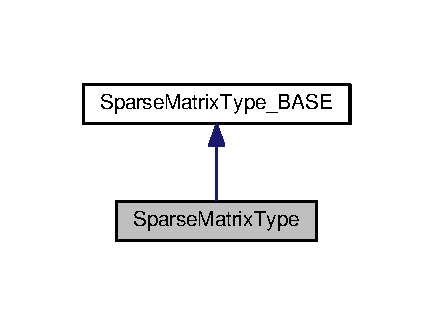
\includegraphics[width=208pt]{class_sparse_matrix_type__inherit__graph}
\end{center}
\end{figure}


Collaboration diagram for Sparse\+Matrix\+Type\+:\nopagebreak
\begin{figure}[H]
\begin{center}
\leavevmode
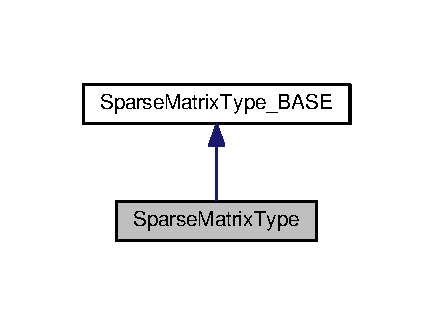
\includegraphics[width=208pt]{class_sparse_matrix_type__coll__graph}
\end{center}
\end{figure}
\subsection*{Public Member Functions}
\begin{DoxyCompactItemize}
\item 
matrix\+\_\+descr \& {\bfseries mkl\+\_\+descr} ()\hypertarget{class_sparse_matrix_type_a1f7a6765acd2ec4fae312ca786962cb9}{}\label{class_sparse_matrix_type_a1f7a6765acd2ec4fae312ca786962cb9}

\item 
sparse\+\_\+matrix\+\_\+t \& {\bfseries mkl\+\_\+matrix} ()\hypertarget{class_sparse_matrix_type_afd47d85a1c895de018cad84451058355}{}\label{class_sparse_matrix_type_afd47d85a1c895de018cad84451058355}

\item 
string {\bfseries matrix\+Type} () const \hypertarget{class_sparse_matrix_type_a5ead28b39f8dfc7688f58b8d39808ef0}{}\label{class_sparse_matrix_type_a5ead28b39f8dfc7688f58b8d39808ef0}

\item 
void {\bfseries Multiply} (const value\+\_\+t a, const value\+\_\+t $\ast$x, const value\+\_\+t b, value\+\_\+t $\ast$y)\hypertarget{class_sparse_matrix_type_ab74d341617d12ed6363db59ee2c7e042}{}\label{class_sparse_matrix_type_ab74d341617d12ed6363db59ee2c7e042}

\item 
void {\bfseries Multiply} (const value\+\_\+t a, const vector\+\_\+t \&x, const value\+\_\+t b, vector\+\_\+t \&y)\hypertarget{class_sparse_matrix_type_af7f5d4236ce2a15d3bc329565f3451cf}{}\label{class_sparse_matrix_type_af7f5d4236ce2a15d3bc329565f3451cf}

\item 
void {\bfseries Rescale} (const value\+\_\+t a, const value\+\_\+t b)\hypertarget{class_sparse_matrix_type_ab99343fb6362ff317669d441c43ab50f}{}\label{class_sparse_matrix_type_ab99343fb6362ff317669d441c43ab50f}

\item 
void {\bfseries Multiply} (const value\+\_\+t $\ast$x, value\+\_\+t $\ast$y)\hypertarget{class_sparse_matrix_type_a3e9ab505f48edce77949dc16f8899674}{}\label{class_sparse_matrix_type_a3e9ab505f48edce77949dc16f8899674}

\item 
void {\bfseries Multiply} (const vector\+\_\+t \&x, vector\+\_\+t \&y)\hypertarget{class_sparse_matrix_type_a7157dab30596a1907e797910039479db}{}\label{class_sparse_matrix_type_a7157dab30596a1907e797910039479db}

\item 
void {\bfseries Batch\+Multiply} (const int batch\+Size, const value\+\_\+t a, const value\+\_\+t $\ast$x, const value\+\_\+t b, value\+\_\+t $\ast$y)\hypertarget{class_sparse_matrix_type_ab708db3441938be5ef65a9450f4af298}{}\label{class_sparse_matrix_type_ab708db3441938be5ef65a9450f4af298}

\item 
void {\bfseries Convert\+From\+C\+OO} (vector$<$ int $>$ \&rows, vector$<$ int $>$ \&cols, vector$<$ complex$<$ double $>$ $>$ \&vals)\hypertarget{class_sparse_matrix_type_aacc74467c65c6370fb335944b3988972}{}\label{class_sparse_matrix_type_aacc74467c65c6370fb335944b3988972}

\item 
void {\bfseries Convert\+From\+C\+SR} (vector$<$ int $>$ \&row\+Index, vector$<$ int $>$ \&cols, vector$<$ complex$<$ double $>$ $>$ \&vals)\hypertarget{class_sparse_matrix_type_a531b65d0596e5044c55be1253fe59559}{}\label{class_sparse_matrix_type_a531b65d0596e5044c55be1253fe59559}

\end{DoxyCompactItemize}
\subsection*{Additional Inherited Members}


The documentation for this class was generated from the following files\+:\begin{DoxyCompactItemize}
\item 
/data/jgarcia/codes/linqt/include/sparse\+\_\+matrix.\+hpp\item 
/data/jgarcia/codes/linqt/src/mkl\+\_\+sparse\+\_\+matrix.\+cpp\end{DoxyCompactItemize}

\hypertarget{class_sparse_matrix_type___b_a_s_e}{}\section{Sparse\+Matrix\+Type\+\_\+\+B\+A\+SE Class Reference}
\label{class_sparse_matrix_type___b_a_s_e}\index{Sparse\+Matrix\+Type\+\_\+\+B\+A\+SE@{Sparse\+Matrix\+Type\+\_\+\+B\+A\+SE}}


Inheritance diagram for Sparse\+Matrix\+Type\+\_\+\+B\+A\+SE\+:\nopagebreak
\begin{figure}[H]
\begin{center}
\leavevmode
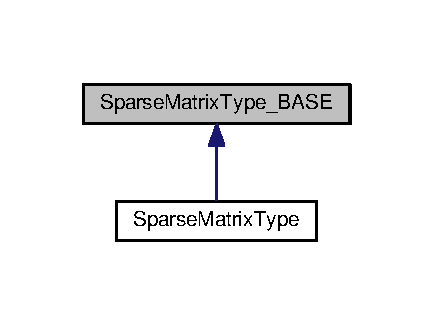
\includegraphics[width=208pt]{class_sparse_matrix_type___b_a_s_e__inherit__graph}
\end{center}
\end{figure}
\subsection*{Public Types}
\begin{DoxyCompactItemize}
\item 
typedef complex$<$ double $>$ {\bfseries value\+\_\+t}\hypertarget{class_sparse_matrix_type___b_a_s_e_a9291ab7ea4ac6d98db8f4debe8e32e1d}{}\label{class_sparse_matrix_type___b_a_s_e_a9291ab7ea4ac6d98db8f4debe8e32e1d}

\item 
typedef vector$<$ value\+\_\+t $>$ {\bfseries vector\+\_\+t}\hypertarget{class_sparse_matrix_type___b_a_s_e_a57c552a5411526c9a46b045c1a47804b}{}\label{class_sparse_matrix_type___b_a_s_e_a57c552a5411526c9a46b045c1a47804b}

\end{DoxyCompactItemize}
\subsection*{Public Member Functions}
\begin{DoxyCompactItemize}
\item 
int {\bfseries num\+Rows} ()\hypertarget{class_sparse_matrix_type___b_a_s_e_aca478d5a5a082ee3deb49ac515f71d29}{}\label{class_sparse_matrix_type___b_a_s_e_aca478d5a5a082ee3deb49ac515f71d29}

\item 
int {\bfseries num\+Cols} ()\hypertarget{class_sparse_matrix_type___b_a_s_e_ae92cdc0b9f2c97499f941ec002b8cfc7}{}\label{class_sparse_matrix_type___b_a_s_e_ae92cdc0b9f2c97499f941ec002b8cfc7}

\item 
int {\bfseries rank} ()\hypertarget{class_sparse_matrix_type___b_a_s_e_acefb2ce1679eea7c79f47acfb368aa22}{}\label{class_sparse_matrix_type___b_a_s_e_acefb2ce1679eea7c79f47acfb368aa22}

\item 
void {\bfseries set\+Dimensions} (const int num\+Rows, const int num\+Cols)\hypertarget{class_sparse_matrix_type___b_a_s_e_a177132ea003e9eb4ae5044786c761e82}{}\label{class_sparse_matrix_type___b_a_s_e_a177132ea003e9eb4ae5044786c761e82}

\item 
void {\bfseries Set\+ID} (string id)\hypertarget{class_sparse_matrix_type___b_a_s_e_a76ea4693a656fe0a8d4c234c517886e7}{}\label{class_sparse_matrix_type___b_a_s_e_a76ea4693a656fe0a8d4c234c517886e7}

\item 
string {\bfseries ID} () const \hypertarget{class_sparse_matrix_type___b_a_s_e_a759bbb1277e60b987445e616f532acf5}{}\label{class_sparse_matrix_type___b_a_s_e_a759bbb1277e60b987445e616f532acf5}

\end{DoxyCompactItemize}


The documentation for this class was generated from the following file\+:\begin{DoxyCompactItemize}
\item 
/data/jgarcia/codes/linqt/include/sparse\+\_\+matrix.\+hpp\end{DoxyCompactItemize}

\hypertarget{classtbmodel}{}\section{tbmodel Class Reference}
\label{classtbmodel}\index{tbmodel@{tbmodel}}


{\ttfamily \#include $<$tbmodel.\+hpp$>$}



Collaboration diagram for tbmodel\+:\nopagebreak
\begin{figure}[H]
\begin{center}
\leavevmode
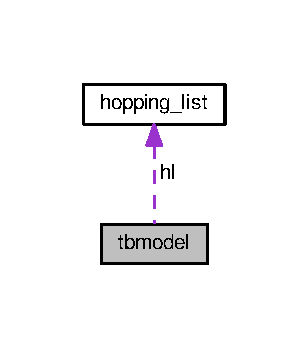
\includegraphics[width=148pt]{classtbmodel__coll__graph}
\end{center}
\end{figure}
\subsection*{Public Types}
\begin{DoxyCompactItemize}
\item 
typedef tuple$<$ string, array$<$ double, 3 $>$ $>$ {\bfseries orb\+Pos\+\_\+t}\hypertarget{classtbmodel_a76dca7d0eb27c0a04cbde93974ae68e8}{}\label{classtbmodel_a76dca7d0eb27c0a04cbde93974ae68e8}

\item 
typedef array$<$ array$<$ double, 3 $>$, 3 $>$ {\bfseries unit\+Cell\+\_\+t}\hypertarget{classtbmodel_a34391d0e7eca0f75360009c5898b8d02}{}\label{classtbmodel_a34391d0e7eca0f75360009c5898b8d02}

\item 
typedef multimap$<$ string, \hyperlink{classhopping__kind}{hopping\+\_\+kind} $>$ {\bfseries hopping\+\_\+kind\+\_\+list}\hypertarget{classtbmodel_ab2715f3f60cd388612806e79e233748c}{}\label{classtbmodel_ab2715f3f60cd388612806e79e233748c}

\end{DoxyCompactItemize}
\subsection*{Public Member Functions}
\begin{DoxyCompactItemize}
\item 
void {\bfseries read\+Unit\+Cell} (const string inputfile)\hypertarget{classtbmodel_adee0ff864c43723c8c979f4e2e008bb6}{}\label{classtbmodel_adee0ff864c43723c8c979f4e2e008bb6}

\item 
void {\bfseries read\+Orbital\+Positions} (const string inputfile)\hypertarget{classtbmodel_a1fce67740fd3fed482cd68357cdb9cbe}{}\label{classtbmodel_a1fce67740fd3fed482cd68357cdb9cbe}

\item 
void {\bfseries read\+Wannier\+Model} (const string inputfile)\hypertarget{classtbmodel_aeef6853760e7ce690be52bc5f52b6e72}{}\label{classtbmodel_aeef6853760e7ce690be52bc5f52b6e72}

\item 
void {\bfseries read\+Static\+Disorder} (const string inputfile)\hypertarget{classtbmodel_af9feab7007f63a5f150a02cc8bcf6fa0}{}\label{classtbmodel_af9feab7007f63a5f150a02cc8bcf6fa0}

\item 
map$<$ int, string $>$ \hyperlink{classtbmodel_a1285d524d1bc13a01ada7e3c401d9e9c}{map\+\_\+id2orbs} ()
\item 
map$<$ int, int $>$ \hyperlink{classtbmodel_a879c46b9c956e0fdeaa7e8f924773c6f}{map\+\_\+id2spin} ()
\item 
\hyperlink{classhopping__list}{hopping\+\_\+list} \& {\bfseries Hopping\+\_\+\+List} ()\hypertarget{classtbmodel_aada1c093588ba10a3a33e493b9264a4a}{}\label{classtbmodel_aada1c093588ba10a3a33e493b9264a4a}

\item 
\hyperlink{classhopping__list}{hopping\+\_\+list} \hyperlink{classtbmodel_aec77e33a90b894377def9814c91ca49d}{create\+Local\+Hopping\+\_\+list} ()
\item 
\hyperlink{classhopping__list}{hopping\+\_\+list} \hyperlink{classtbmodel_aec3324656e65583ec29f935757b4bc2e}{create\+Hopping\+Density\+\_\+list} (\hyperlink{structoputil_1_1op__matrix}{oputil\+::op\+\_\+matrix} OP)
\item 
\hyperlink{classhopping__list}{hopping\+\_\+list} \hyperlink{classtbmodel_a77324c81674f2c43e6214ca8313ced79}{create\+Hopping\+Currents\+\_\+list} (const int dir)
\item 
\hyperlink{classhopping__list}{hopping\+\_\+list} \hyperlink{classtbmodel_aae40bea134fc6d634cc82a0bf2cb0a5d}{create\+Hopping\+Spin\+Density\+\_\+list} (const double theta, const double phi)
\item 
\hyperlink{classhopping__list}{hopping\+\_\+list} \hyperlink{classtbmodel_ab9766c523ec0221ac91ccd507ed8f992}{create\+Hopping\+Torque\+Density\+\_\+list} (const double theta, const double phi)
\item 
\hyperlink{classhopping__list}{hopping\+\_\+list} \hyperlink{classtbmodel_a31f942be44b0a1af276ba413276d046e}{create\+Hopping\+Spin\+Currents\+\_\+list} (const int dir, const double theta, const double phi)
\item 
\hyperlink{classhopping__list}{hopping\+\_\+list} {\bfseries create\+Hopping\+Currents\+\_\+list} (const std\+::string op)\hypertarget{classtbmodel_a497b3607c1d498285d68ff08ac2f315b}{}\label{classtbmodel_a497b3607c1d498285d68ff08ac2f315b}

\item 
\hyperlink{classhopping__list}{hopping\+\_\+list} {\bfseries create\+Hopping\+Spinorial\+Density\+\_\+list} (const std\+::array$<$ std\+::complex$<$ double $>$, 4 $>$ op)\hypertarget{classtbmodel_abd021ce1ebe29c77197857eda7641dac}{}\label{classtbmodel_abd021ce1ebe29c77197857eda7641dac}

\item 
\hyperlink{classhopping__list}{hopping\+\_\+list} {\bfseries create\+Hopping\+Spin\+Density\+\_\+list} (const std\+::string op)\hypertarget{classtbmodel_aaf0f711704f7dcfc6f186c97ec024f63}{}\label{classtbmodel_aaf0f711704f7dcfc6f186c97ec024f63}

\item 
\hyperlink{classhopping__list}{hopping\+\_\+list} {\bfseries create\+Hopping\+Torque\+Density\+\_\+list} (const std\+::string op)\hypertarget{classtbmodel_acac9ec7ef9b8e684372e09b14b73aa59}{}\label{classtbmodel_acac9ec7ef9b8e684372e09b14b73aa59}

\item 
\hyperlink{classhopping__list}{hopping\+\_\+list} {\bfseries create\+Hopping\+Spin\+Currents\+\_\+list} (string op)\hypertarget{classtbmodel_a60707b51717f19e59be4876696263c08}{}\label{classtbmodel_a60707b51717f19e59be4876696263c08}

\item 
\hyperlink{classhopping__list}{hopping\+\_\+list} {\bfseries create\+Hopping\+Spin\+Currents\+\_\+list} (const int dir, const char sdir)\hypertarget{classtbmodel_aaad3f86a13ac29afdb6d6c6cd1e9d431}{}\label{classtbmodel_aaad3f86a13ac29afdb6d6c6cd1e9d431}

\item 
\hyperlink{classhopping__list}{hopping\+\_\+list} {\bfseries Wannier\+Operator} (std\+::string op\+\_\+id)\hypertarget{classtbmodel_aabcd375bbfa508596bb233012f9f2a03}{}\label{classtbmodel_aabcd375bbfa508596bb233012f9f2a03}

\item 
void {\bfseries get\+Spin\+Index} (const int \&n, int \&s) const \hypertarget{classtbmodel_a5e74702b6bb666df50783887f50e34c2}{}\label{classtbmodel_a5e74702b6bb666df50783887f50e34c2}

\item 
int {\bfseries get\+Spin\+Index} (const int \&n) const \hypertarget{classtbmodel_adfedf8e29bd8919448a16dc820ef60ed}{}\label{classtbmodel_adfedf8e29bd8919448a16dc820ef60ed}

\end{DoxyCompactItemize}
\subsection*{Public Attributes}
\begin{DoxyCompactItemize}
\item 
int {\bfseries num\+\_\+orbs}\hypertarget{classtbmodel_a6401dfc2dba0df5409a92c069e1de0f0}{}\label{classtbmodel_a6401dfc2dba0df5409a92c069e1de0f0}

\item 
unit\+Cell\+\_\+t {\bfseries lat\+\_\+vecs}\hypertarget{classtbmodel_a2837b8aab16e5e679302894609b7f7af}{}\label{classtbmodel_a2837b8aab16e5e679302894609b7f7af}

\item 
vector$<$ orb\+Pos\+\_\+t $>$ {\bfseries orb\+Pos\+\_\+list}\hypertarget{classtbmodel_ae7d346cc58028b41581412751a16a87f}{}\label{classtbmodel_ae7d346cc58028b41581412751a16a87f}

\item 
\hyperlink{classhopping__list}{hopping\+\_\+list} {\bfseries hl}\hypertarget{classtbmodel_acf3031a7eed087a88ec733bc4ea2df9f}{}\label{classtbmodel_acf3031a7eed087a88ec733bc4ea2df9f}

\end{DoxyCompactItemize}


\subsection{Detailed Description}
The tbmodel class This class is responsible for reading wannier files and converting it into a \hyperlink{classhopping__list}{hopping\+\_\+list} structure It is also responsible for constructing other tight-\/binding operators 

\subsection{Member Function Documentation}
\index{tbmodel@{tbmodel}!create\+Hopping\+Currents\+\_\+list@{create\+Hopping\+Currents\+\_\+list}}
\index{create\+Hopping\+Currents\+\_\+list@{create\+Hopping\+Currents\+\_\+list}!tbmodel@{tbmodel}}
\subsubsection[{\texorpdfstring{create\+Hopping\+Currents\+\_\+list(const int dir)}{createHoppingCurrents_list(const int dir)}}]{\setlength{\rightskip}{0pt plus 5cm}{\bf hopping\+\_\+list} tbmodel\+::create\+Hopping\+Currents\+\_\+list (
\begin{DoxyParamCaption}
\item[{const int}]{dir}
\end{DoxyParamCaption}
)}\hypertarget{classtbmodel_a77324c81674f2c43e6214ca8313ced79}{}\label{classtbmodel_a77324c81674f2c43e6214ca8313ced79}
Construct the current operator for the hopping list. In this context, a current operator is defined as \{i,j\} $\vert$i$>$$<$j$\vert$ I$\ast$\+H\+\_\+\{i,j\}$\ast$(R\+\_\+i-\/\+R\+\_\+j)\+\_\+dir with $\vert$i$>$ the basis vector in which the hoppings $<$i$\vert$\+H$\vert$j$>$ are defined. Here i represents both orbital and unit cell indexes. and d, representes the direction in which you want the current

\begin{DoxyReturn}{Returns}
current\+\_\+hopping\+\_\+list Returns the current operator in the format of a hopping list. 
\end{DoxyReturn}

\begin{DoxyParams}[1]{Parameters}
\mbox{\tt in}  & {\em Direction.} & The direction in which you want the current. \\
\hline
\end{DoxyParams}
\index{tbmodel@{tbmodel}!create\+Hopping\+Density\+\_\+list@{create\+Hopping\+Density\+\_\+list}}
\index{create\+Hopping\+Density\+\_\+list@{create\+Hopping\+Density\+\_\+list}!tbmodel@{tbmodel}}
\subsubsection[{\texorpdfstring{create\+Hopping\+Density\+\_\+list(oputil\+::op\+\_\+matrix O\+P)}{createHoppingDensity_list(oputil::op_matrix OP)}}]{\setlength{\rightskip}{0pt plus 5cm}{\bf hopping\+\_\+list} tbmodel\+::create\+Hopping\+Density\+\_\+list (
\begin{DoxyParamCaption}
\item[{{\bf oputil\+::op\+\_\+matrix}}]{OP}
\end{DoxyParamCaption}
)}\hypertarget{classtbmodel_aec3324656e65583ec29f935757b4bc2e}{}\label{classtbmodel_aec3324656e65583ec29f935757b4bc2e}
Construct a density operator for the hopping list an a matrix defining an operator. In this context, the matrix is defined only in the unit cell, hereby the reason for calling it a density operator. The density operator is then defined as \{i in cell\} M\+\_\+ij$\vert$i$>$$<$j$\vert$ with $\vert$i$>$ the basis vector in which the hoppings $<$i,0,0,0$\vert$\+H$\vert$j,0,0,0$>$ are defined. The (0,0,0) indexes is to note that this operator only consider hoppings within the unit cell \begin{DoxyReturn}{Returns}
density\+\_\+hopping\+\_\+list Returns the density operator in the format of a hopping list. 
\end{DoxyReturn}
\index{tbmodel@{tbmodel}!create\+Hopping\+Spin\+Currents\+\_\+list@{create\+Hopping\+Spin\+Currents\+\_\+list}}
\index{create\+Hopping\+Spin\+Currents\+\_\+list@{create\+Hopping\+Spin\+Currents\+\_\+list}!tbmodel@{tbmodel}}
\subsubsection[{\texorpdfstring{create\+Hopping\+Spin\+Currents\+\_\+list(const int dir, const double theta, const double phi)}{createHoppingSpinCurrents_list(const int dir, const double theta, const double phi)}}]{\setlength{\rightskip}{0pt plus 5cm}{\bf hopping\+\_\+list} tbmodel\+::create\+Hopping\+Spin\+Currents\+\_\+list (
\begin{DoxyParamCaption}
\item[{const int}]{dir, }
\item[{const double}]{theta, }
\item[{const double}]{phi}
\end{DoxyParamCaption}
)}\hypertarget{classtbmodel_a31f942be44b0a1af276ba413276d046e}{}\label{classtbmodel_a31f942be44b0a1af276ba413276d046e}
Construct the current density operator in the direction u = ( sin(theta)$\ast$cos(phi),sin(theta)$\ast$sin(phi), cos(theta) );

\begin{DoxyReturn}{Returns}
spin\+\_\+current density\+\_\+hopping\+\_\+list Returns the Current Density operator in the format of a hopping list. 
\end{DoxyReturn}

\begin{DoxyParams}[1]{Parameters}
\mbox{\tt in}  & {\em Theta.} & angle defining the altitute direction in which you want the current. \\
\hline
\mbox{\tt in}  & {\em Phi.} & angle defining the azimuth \\
\hline
\end{DoxyParams}
\index{tbmodel@{tbmodel}!create\+Hopping\+Spin\+Density\+\_\+list@{create\+Hopping\+Spin\+Density\+\_\+list}}
\index{create\+Hopping\+Spin\+Density\+\_\+list@{create\+Hopping\+Spin\+Density\+\_\+list}!tbmodel@{tbmodel}}
\subsubsection[{\texorpdfstring{create\+Hopping\+Spin\+Density\+\_\+list(const double theta, const double phi)}{createHoppingSpinDensity_list(const double theta, const double phi)}}]{\setlength{\rightskip}{0pt plus 5cm}{\bf hopping\+\_\+list} tbmodel\+::create\+Hopping\+Spin\+Density\+\_\+list (
\begin{DoxyParamCaption}
\item[{const double}]{theta, }
\item[{const double}]{phi}
\end{DoxyParamCaption}
)}\hypertarget{classtbmodel_aae40bea134fc6d634cc82a0bf2cb0a5d}{}\label{classtbmodel_aae40bea134fc6d634cc82a0bf2cb0a5d}
Construct the density operator in the direction u = ( sin(theta)$\ast$cos(phi),sin(theta)$\ast$sin(phi), cos(theta); In this context, OP = Su, the spin direction.

\begin{DoxyReturn}{Returns}
density\+\_\+hopping\+\_\+list Returns the density operator in the format of a hopping list. 
\end{DoxyReturn}

\begin{DoxyParams}[1]{Parameters}
\mbox{\tt in}  & {\em Theta.} & angle defining the altitute direction in which you want the current. \\
\hline
\mbox{\tt in}  & {\em Phi.} & angle defining the azimuth \\
\hline
\end{DoxyParams}
\index{tbmodel@{tbmodel}!create\+Hopping\+Torque\+Density\+\_\+list@{create\+Hopping\+Torque\+Density\+\_\+list}}
\index{create\+Hopping\+Torque\+Density\+\_\+list@{create\+Hopping\+Torque\+Density\+\_\+list}!tbmodel@{tbmodel}}
\subsubsection[{\texorpdfstring{create\+Hopping\+Torque\+Density\+\_\+list(const double theta, const double phi)}{createHoppingTorqueDensity_list(const double theta, const double phi)}}]{\setlength{\rightskip}{0pt plus 5cm}{\bf hopping\+\_\+list} tbmodel\+::create\+Hopping\+Torque\+Density\+\_\+list (
\begin{DoxyParamCaption}
\item[{const double}]{theta, }
\item[{const double}]{phi}
\end{DoxyParamCaption}
)}\hypertarget{classtbmodel_ab9766c523ec0221ac91ccd507ed8f992}{}\label{classtbmodel_ab9766c523ec0221ac91ccd507ed8f992}
Construct the density operator in the direction u = ( sin(theta)$\ast$cos(phi),sin(theta)$\ast$sin(phi), cos(theta); In this context, OP = Su, the spin direction.

\begin{DoxyReturn}{Returns}
density\+\_\+hopping\+\_\+list Returns the density operator in the format of a hopping list. 
\end{DoxyReturn}

\begin{DoxyParams}[1]{Parameters}
\mbox{\tt in}  & {\em Theta.} & angle defining the altitute direction in which you want the current. \\
\hline
\mbox{\tt in}  & {\em Phi.} & angle defining the azimuth \\
\hline
\end{DoxyParams}
\index{tbmodel@{tbmodel}!create\+Local\+Hopping\+\_\+list@{create\+Local\+Hopping\+\_\+list}}
\index{create\+Local\+Hopping\+\_\+list@{create\+Local\+Hopping\+\_\+list}!tbmodel@{tbmodel}}
\subsubsection[{\texorpdfstring{create\+Local\+Hopping\+\_\+list()}{createLocalHopping_list()}}]{\setlength{\rightskip}{0pt plus 5cm}{\bf hopping\+\_\+list} tbmodel\+::create\+Local\+Hopping\+\_\+list (
\begin{DoxyParamCaption}
{}
\end{DoxyParamCaption}
)}\hypertarget{classtbmodel_aec77e33a90b894377def9814c91ca49d}{}\label{classtbmodel_aec77e33a90b894377def9814c91ca49d}
Extract the local hoppings for the hopping list. In this context, the local hoppings are the one satisfying \{i in cell\} H\+\_\+ij$\vert$i$>$$<$j$\vert$ with $\vert$i$>$ the basis vector in which the hoppings $<$i,0,0,0$\vert$\+H$\vert$j,0,0,0$>$ are defined. The (0,0,0) indexes is to note that this operator only consider hoppings within the unit cell \begin{DoxyReturn}{Returns}
density\+\_\+hopping\+\_\+list Returns the density operator in the format of a hopping list. 
\end{DoxyReturn}
\index{tbmodel@{tbmodel}!map\+\_\+id2orbs@{map\+\_\+id2orbs}}
\index{map\+\_\+id2orbs@{map\+\_\+id2orbs}!tbmodel@{tbmodel}}
\subsubsection[{\texorpdfstring{map\+\_\+id2orbs()}{map_id2orbs()}}]{\setlength{\rightskip}{0pt plus 5cm}map$<$ int, string $>$ tbmodel\+::map\+\_\+id2orbs (
\begin{DoxyParamCaption}
{}
\end{DoxyParamCaption}
)}\hypertarget{classtbmodel_a1285d524d1bc13a01ada7e3c401d9e9c}{}\label{classtbmodel_a1285d524d1bc13a01ada7e3c401d9e9c}
Transform a site tag into real space cartesian vector.


\begin{DoxyParams}[1]{Parameters}
\mbox{\tt out}  & {\em cart\+\_\+vect.} & A three-\/dimensional real vector, constructed from the tag and the lattice vectors \\
\hline
\mbox{\tt in}  & {\em tag.} & An identification of the position of a unit cell. In this version of the code, this is the position in units of lattice vector. \\
\hline
\mbox{\tt in}  & {\em lattice\+\_\+vector.} & The set of lattice vectors \\
\hline
\end{DoxyParams}
\index{tbmodel@{tbmodel}!map\+\_\+id2spin@{map\+\_\+id2spin}}
\index{map\+\_\+id2spin@{map\+\_\+id2spin}!tbmodel@{tbmodel}}
\subsubsection[{\texorpdfstring{map\+\_\+id2spin()}{map_id2spin()}}]{\setlength{\rightskip}{0pt plus 5cm}map$<$ int, int $>$ tbmodel\+::map\+\_\+id2spin (
\begin{DoxyParamCaption}
{}
\end{DoxyParamCaption}
)}\hypertarget{classtbmodel_a879c46b9c956e0fdeaa7e8f924773c6f}{}\label{classtbmodel_a879c46b9c956e0fdeaa7e8f924773c6f}
Transform a site tag into real space cartesian vector.


\begin{DoxyParams}[1]{Parameters}
\mbox{\tt out}  & {\em cart\+\_\+vect.} & A three-\/dimensional real vector, constructed from the tag and the lattice vectors \\
\hline
\mbox{\tt in}  & {\em tag.} & An identification of the position of a unit cell. In this version of the code, this is the position in units of lattice vector. \\
\hline
\mbox{\tt in}  & {\em lattice\+\_\+vector.} & The set of lattice vectors \\
\hline
\end{DoxyParams}


The documentation for this class was generated from the following files\+:\begin{DoxyCompactItemize}
\item 
/data/jgarcia/codes/linqt/utilities/wannier2sparse/include/tbmodel.\+hpp\item 
/data/jgarcia/codes/linqt/utilities/wannier2sparse/src/tbmodel.\+cpp\end{DoxyCompactItemize}

\hypertarget{class_vector_list}{}\section{Vector\+List$<$ T $>$ Class Template Reference}
\label{class_vector_list}\index{Vector\+List$<$ T $>$@{Vector\+List$<$ T $>$}}
\subsection*{Public Types}
\begin{DoxyCompactItemize}
\item 
typedef vector$<$ T $>$ {\bfseries vector\+\_\+t}\hypertarget{class_vector_list_a4ef3e8b689d699aff1ba43ebca715297}{}\label{class_vector_list_a4ef3e8b689d699aff1ba43ebca715297}

\item 
typedef vector$<$ vector\+\_\+t $>$ {\bfseries list\+\_\+t}\hypertarget{class_vector_list_ab5c30ed2bba0842a4ceac36c74d1bfe5}{}\label{class_vector_list_ab5c30ed2bba0842a4ceac36c74d1bfe5}

\end{DoxyCompactItemize}
\subsection*{Public Member Functions}
\begin{DoxyCompactItemize}
\item 
{\bfseries Vector\+List} (size\+\_\+t list\+\_\+count, size\+\_\+t count, const T value=T(0))\hypertarget{class_vector_list_a0837ae6e888fb3876c8fcb0ad8049e1c}{}\label{class_vector_list_a0837ae6e888fb3876c8fcb0ad8049e1c}

\item 
size\+\_\+t {\bfseries Vector\+Size} () const \hypertarget{class_vector_list_a2c6b87ee550f3b6114eb0df2a0897c35}{}\label{class_vector_list_a2c6b87ee550f3b6114eb0df2a0897c35}

\item 
size\+\_\+t {\bfseries List\+Size} () const \hypertarget{class_vector_list_a07e32900bf03659c8e047d2f9151795b}{}\label{class_vector_list_a07e32900bf03659c8e047d2f9151795b}

\item 
list\+\_\+t \& {\bfseries List} ()\hypertarget{class_vector_list_ad504acb2a162836ff421c45e36890f9b}{}\label{class_vector_list_ad504acb2a162836ff421c45e36890f9b}

\item 
vector\+\_\+t \& {\bfseries List\+Elem} (const size\+\_\+t i)\hypertarget{class_vector_list_a72945ca5e0745ede97c9f3193492f908}{}\label{class_vector_list_a72945ca5e0745ede97c9f3193492f908}

\item 
T \& {\bfseries operator()} (const size\+\_\+t i, const size\+\_\+t j)\hypertarget{class_vector_list_a02ed6a307417d9fcb40d1402922058f2}{}\label{class_vector_list_a02ed6a307417d9fcb40d1402922058f2}

\end{DoxyCompactItemize}


The documentation for this class was generated from the following file\+:\begin{DoxyCompactItemize}
\item 
/data/jgarcia/codes/linqt/include/vector\+\_\+list.\+hpp\end{DoxyCompactItemize}

\hypertarget{classchebyshev_1_1_vectors}{}\section{chebyshev\+:\+:Vectors Class Reference}
\label{classchebyshev_1_1_vectors}\index{chebyshev\+::\+Vectors@{chebyshev\+::\+Vectors}}


Inheritance diagram for chebyshev\+:\+:Vectors\+:\nopagebreak
\begin{figure}[H]
\begin{center}
\leavevmode
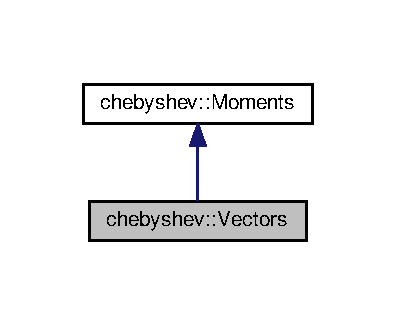
\includegraphics[width=190pt]{classchebyshev_1_1_vectors__inherit__graph}
\end{center}
\end{figure}


Collaboration diagram for chebyshev\+:\+:Vectors\+:\nopagebreak
\begin{figure}[H]
\begin{center}
\leavevmode
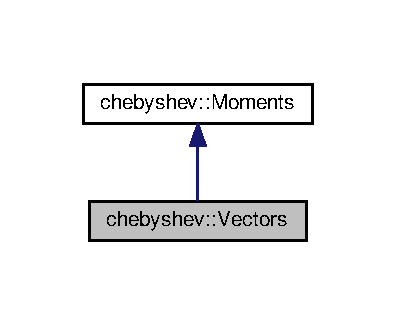
\includegraphics[width=190pt]{classchebyshev_1_1_vectors__coll__graph}
\end{center}
\end{figure}
\subsection*{Public Types}
\begin{DoxyCompactItemize}
\item 
typedef \hyperlink{class_vector_list}{Vector\+List}$<$ Moments\+::value\+\_\+t $>$ {\bfseries vector\+List\+\_\+t}\hypertarget{classchebyshev_1_1_vectors_a1a6e132ce26c89c86e3c1d2df240cdad}{}\label{classchebyshev_1_1_vectors_a1a6e132ce26c89c86e3c1d2df240cdad}

\end{DoxyCompactItemize}
\subsection*{Public Member Functions}
\begin{DoxyCompactItemize}
\item 
{\bfseries Vectors} (const size\+\_\+t n\+Moms, const size\+\_\+t dim)\hypertarget{classchebyshev_1_1_vectors_a47bceab1fdf23555a7da246983a799d8}{}\label{classchebyshev_1_1_vectors_a47bceab1fdf23555a7da246983a799d8}

\item 
{\bfseries Vectors} (\hyperlink{classchebyshev_1_1_moments1_d}{Moments1D} mom)\hypertarget{classchebyshev_1_1_vectors_a35d85ed43200417dea2e698c09766a43}{}\label{classchebyshev_1_1_vectors_a35d85ed43200417dea2e698c09766a43}

\item 
{\bfseries Vectors} (\hyperlink{classchebyshev_1_1_moments2_d}{Moments2D} mom)\hypertarget{classchebyshev_1_1_vectors_aa11abf4e8251b6a9b69d56191a653844}{}\label{classchebyshev_1_1_vectors_aa11abf4e8251b6a9b69d56191a653844}

\item 
{\bfseries Vectors} (\hyperlink{classchebyshev_1_1_moments2_d}{Moments2D} mom, const size\+\_\+t i)\hypertarget{classchebyshev_1_1_vectors_a9cee99d5d80da73abeec40f96568ade1}{}\label{classchebyshev_1_1_vectors_a9cee99d5d80da73abeec40f96568ade1}

\item 
{\bfseries Vectors} (\hyperlink{classchebyshev_1_1_moments_t_d}{Moments\+TD} mom)\hypertarget{classchebyshev_1_1_vectors_ad922ad16003b2526c71898b122688b65}{}\label{classchebyshev_1_1_vectors_ad922ad16003b2526c71898b122688b65}

\item 
size\+\_\+t {\bfseries Size} () const \hypertarget{classchebyshev_1_1_vectors_a30dc46a183c087fac30a3bc4d78b1094}{}\label{classchebyshev_1_1_vectors_a30dc46a183c087fac30a3bc4d78b1094}

\item 
size\+\_\+t {\bfseries System\+Size} () const \hypertarget{classchebyshev_1_1_vectors_a23d0d7c8fba9f9819d3aef9b0d9d9163}{}\label{classchebyshev_1_1_vectors_a23d0d7c8fba9f9819d3aef9b0d9d9163}

\item 
size\+\_\+t {\bfseries Highest\+Moment\+Number} () const \hypertarget{classchebyshev_1_1_vectors_a08aea691c50843f1a797cf09b624a9e2}{}\label{classchebyshev_1_1_vectors_a08aea691c50843f1a797cf09b624a9e2}

\item 
\hyperlink{class_vector_list}{vector\+List\+\_\+t} \& {\bfseries List} ()\hypertarget{classchebyshev_1_1_vectors_adf7b1351546490cbf11619cbaa49ffb6}{}\label{classchebyshev_1_1_vectors_adf7b1351546490cbf11619cbaa49ffb6}

\item 
Moments\+::vector\+\_\+t \& {\bfseries Vector} (const size\+\_\+t m0)\hypertarget{classchebyshev_1_1_vectors_ad7fb30e4b0200f4c3bc4e6f9528c1139}{}\label{classchebyshev_1_1_vectors_ad7fb30e4b0200f4c3bc4e6f9528c1139}

\item 
Moments\+::value\+\_\+t \& {\bfseries operator()} (const size\+\_\+t m0)\hypertarget{classchebyshev_1_1_vectors_a017a8ee693aa4d9f206a541872d2d117}{}\label{classchebyshev_1_1_vectors_a017a8ee693aa4d9f206a541872d2d117}

\item 
int {\bfseries Iterate\+All} (\hyperlink{class_sparse_matrix_type}{Sparse\+Matrix\+Type} \&N\+H\+AM)\hypertarget{classchebyshev_1_1_vectors_a189bb070d0310aa8dede2721c2df189f}{}\label{classchebyshev_1_1_vectors_a189bb070d0310aa8dede2721c2df189f}

\item 
int {\bfseries Evolve\+All} (\hyperlink{class_sparse_matrix_type}{Sparse\+Matrix\+Type} \&N\+H\+AM, const double DeltaT, const double Omega0)\hypertarget{classchebyshev_1_1_vectors_aec0080410aaab617e2a491be414824c0}{}\label{classchebyshev_1_1_vectors_aec0080410aaab617e2a491be414824c0}

\item 
int {\bfseries Multiply} (\hyperlink{class_sparse_matrix_type}{Sparse\+Matrix\+Type} \&OP)\hypertarget{classchebyshev_1_1_vectors_a006a4bbef4757065613daf41d6d22bee}{}\label{classchebyshev_1_1_vectors_a006a4bbef4757065613daf41d6d22bee}

\item 
double {\bfseries Memory\+Consumption\+In\+GB} ()\hypertarget{classchebyshev_1_1_vectors_a843740c964a4e430a5e832fac8e6dc9d}{}\label{classchebyshev_1_1_vectors_a843740c964a4e430a5e832fac8e6dc9d}

\end{DoxyCompactItemize}


The documentation for this class was generated from the following files\+:\begin{DoxyCompactItemize}
\item 
/data/jgarcia/codes/linqt/include/chebyshev\+\_\+moments.\+hpp\item 
/data/jgarcia/codes/linqt/src/chebyshev\+\_\+vectors.\+cpp\end{DoxyCompactItemize}

\hypertarget{class_w2_s_p__arguments}{}\section{W2\+S\+P\+\_\+arguments Class Reference}
\label{class_w2_s_p__arguments}\index{W2\+S\+P\+\_\+arguments@{W2\+S\+P\+\_\+arguments}}


{\ttfamily \#include $<$w2sp\+\_\+arguments.\+hpp$>$}

\subsection*{Public Member Functions}
\begin{DoxyCompactItemize}
\item 
int {\bfseries Read\+Arguments} (int argc, char $\ast$argv\mbox{[}$\,$\mbox{]})\hypertarget{class_w2_s_p__arguments_afe339aa7b9ece593138992383d0d7df2}{}\label{class_w2_s_p__arguments_afe339aa7b9ece593138992383d0d7df2}

\end{DoxyCompactItemize}
\subsection*{Public Attributes}
\begin{DoxyCompactItemize}
\item 
array$<$ int, 3 $>$ {\bfseries cell\+Dim}\hypertarget{class_w2_s_p__arguments_a46d91dbcde18e388672e5587bdb0e243}{}\label{class_w2_s_p__arguments_a46d91dbcde18e388672e5587bdb0e243}

\item 
string {\bfseries label}\hypertarget{class_w2_s_p__arguments_a8033248c369be266bec4f668264bf183}{}\label{class_w2_s_p__arguments_a8033248c369be266bec4f668264bf183}

\item 
string {\bfseries program\+\_\+name}\hypertarget{class_w2_s_p__arguments_a92f67e03c019035d66f6d74d592e121d}{}\label{class_w2_s_p__arguments_a92f67e03c019035d66f6d74d592e121d}

\item 
string {\bfseries current\+\_\+error}\hypertarget{class_w2_s_p__arguments_aa327835490b77458d1157f8a83b05ec3}{}\label{class_w2_s_p__arguments_aa327835490b77458d1157f8a83b05ec3}

\item 
deque$<$ string $>$ {\bfseries arguments}\hypertarget{class_w2_s_p__arguments_a95f44f50a04111000da2a893731d2437}{}\label{class_w2_s_p__arguments_a95f44f50a04111000da2a893731d2437}

\item 
deque$<$ string $>$ {\bfseries operators}\hypertarget{class_w2_s_p__arguments_a0ee2f27ace415c94334bc5a0211bd4ec}{}\label{class_w2_s_p__arguments_a0ee2f27ace415c94334bc5a0211bd4ec}

\end{DoxyCompactItemize}


\subsection{Detailed Description}
This is a class which has as main role to handle input arguments of the program. It should\+: (a) Read and validate the arguments from a command line. Done (b) Read and validate the arguments from a config file. Done 

The documentation for this class was generated from the following file\+:\begin{DoxyCompactItemize}
\item 
/data/jgarcia/codes/linqt/utilities/wannier2sparse/include/w2sp\+\_\+arguments.\+hpp\end{DoxyCompactItemize}

\hypertarget{classwannier__tools_1_1wannier__system}{}\section{wannier\+\_\+tools.\+wannier\+\_\+system Class Reference}
\label{classwannier__tools_1_1wannier__system}\index{wannier\+\_\+tools.\+wannier\+\_\+system@{wannier\+\_\+tools.\+wannier\+\_\+system}}
\subsection*{Public Member Functions}
\begin{DoxyCompactItemize}
\item 
def {\bfseries \+\_\+\+\_\+init\+\_\+\+\_\+} (self, label)\hypertarget{classwannier__tools_1_1wannier__system_a151284373ee50c477a6815a1f4487195}{}\label{classwannier__tools_1_1wannier__system_a151284373ee50c477a6815a1f4487195}

\item 
def {\bfseries load\+\_\+xyz} (self, filename)\hypertarget{classwannier__tools_1_1wannier__system_a845c993eb3dc8ddbce05062883d5b1f1}{}\label{classwannier__tools_1_1wannier__system_a845c993eb3dc8ddbce05062883d5b1f1}

\item 
def {\bfseries load\+\_\+wannier\+\_\+file} (self, filename)\hypertarget{classwannier__tools_1_1wannier__system_a0ae2338ce73e8b0fd08ffbf4c462aefb}{}\label{classwannier__tools_1_1wannier__system_a0ae2338ce73e8b0fd08ffbf4c462aefb}

\item 
def {\bfseries spin\+\_\+operator} (self, comp=None)\hypertarget{classwannier__tools_1_1wannier__system_a54cc2f95c64dc0ba5bcffbc2543179bb}{}\label{classwannier__tools_1_1wannier__system_a54cc2f95c64dc0ba5bcffbc2543179bb}

\item 
def {\bfseries ham\+\_\+operator} (self, k)\hypertarget{classwannier__tools_1_1wannier__system_a6df5aaa2172f2da72d1a6d49f2c3206e}{}\label{classwannier__tools_1_1wannier__system_a6df5aaa2172f2da72d1a6d49f2c3206e}

\item 
def {\bfseries projected\+\_\+eigenvalues} (self, k, proj\+\_\+op)\hypertarget{classwannier__tools_1_1wannier__system_a2a79f28a672e647403e037afe921f250}{}\label{classwannier__tools_1_1wannier__system_a2a79f28a672e647403e037afe921f250}

\item 
def {\bfseries Momentum\+\_\+\+Rec2\+Abs\+Matrix} (self)\hypertarget{classwannier__tools_1_1wannier__system_a08086c7ac54b43f0a6add1ab0c2154c0}{}\label{classwannier__tools_1_1wannier__system_a08086c7ac54b43f0a6add1ab0c2154c0}

\item 
def {\bfseries to\+Absolute\+Coords} (self, x)\hypertarget{classwannier__tools_1_1wannier__system_a8ce7c9888adbe63bda90bc12d8fa2509}{}\label{classwannier__tools_1_1wannier__system_a8ce7c9888adbe63bda90bc12d8fa2509}

\item 
def {\bfseries band\+\_\+kpoints} (self, absolute\+\_\+coords=False)\hypertarget{classwannier__tools_1_1wannier__system_a3c3e556974ac41c6395be85c10765c94}{}\label{classwannier__tools_1_1wannier__system_a3c3e556974ac41c6395be85c10765c94}

\item 
def {\bfseries set\+\_\+bandpath} (self, bandpath, absolute\+\_\+coords=False)\hypertarget{classwannier__tools_1_1wannier__system_a202eba5a09b7fda11184fb59fc8965eb}{}\label{classwannier__tools_1_1wannier__system_a202eba5a09b7fda11184fb59fc8965eb}

\item 
def {\bfseries get\+\_\+\+X\+Labels} (self)\hypertarget{classwannier__tools_1_1wannier__system_af7219ab9427179e77c5cdb506b0ee8d2}{}\label{classwannier__tools_1_1wannier__system_af7219ab9427179e77c5cdb506b0ee8d2}

\item 
def {\bfseries bands\+Xaxis} (self)\hypertarget{classwannier__tools_1_1wannier__system_a8e86c1865dc5a8b18e27b9a8da5c9bb7}{}\label{classwannier__tools_1_1wannier__system_a8e86c1865dc5a8b18e27b9a8da5c9bb7}

\item 
def {\bfseries compute\+\_\+band\+\_\+structure} (self, fermi\+\_\+energy=0.\+0, proj\+\_\+op=None, ax=None, plot\+\_\+proj=False, proj\+\_\+range=None)\hypertarget{classwannier__tools_1_1wannier__system_a52cfe2e57e3ecf3b2da0c9b3a7a68bc6}{}\label{classwannier__tools_1_1wannier__system_a52cfe2e57e3ecf3b2da0c9b3a7a68bc6}

\item 
def {\bfseries plot\+\_\+band\+\_\+structure} (self, bands, projs=None, ax=None, plot\+\_\+proj=False, proj\+\_\+range=None)\hypertarget{classwannier__tools_1_1wannier__system_a065a5c97b9369c76a6f86988d9b414b1}{}\label{classwannier__tools_1_1wannier__system_a065a5c97b9369c76a6f86988d9b414b1}

\item 
def {\bfseries compute\+\_\+dispersion} (self, kpoints, proj\+\_\+op=None)\hypertarget{classwannier__tools_1_1wannier__system_a8ce170e12aec3bed3b717805c4500796}{}\label{classwannier__tools_1_1wannier__system_a8ce170e12aec3bed3b717805c4500796}

\item 
def {\bfseries compute\+\_\+fermi\+\_\+surface} (self, kpoints, fermi\+\_\+energy=0.\+0, tol=None, proj\+\_\+op=None)\hypertarget{classwannier__tools_1_1wannier__system_ad48d42d6bcce91039211596875f092a7}{}\label{classwannier__tools_1_1wannier__system_ad48d42d6bcce91039211596875f092a7}

\item 
def {\bfseries refine\+\_\+kpoints} (self, kpoints)\hypertarget{classwannier__tools_1_1wannier__system_a774d5a49d1ad4d7e7f4932312a6605fc}{}\label{classwannier__tools_1_1wannier__system_a774d5a49d1ad4d7e7f4932312a6605fc}

\item 
def {\bfseries compute\+\_\+\+D\+OS} (self, energies, gridpoints, fermi\+\_\+energy=0.\+0, broadening=0.\+1, kpoints=None, proj\+\_\+op=None)\hypertarget{classwannier__tools_1_1wannier__system_a3df841935dde3452689cea1c3f26724a}{}\label{classwannier__tools_1_1wannier__system_a3df841935dde3452689cea1c3f26724a}

\end{DoxyCompactItemize}
\subsection*{Public Attributes}
\begin{DoxyCompactItemize}
\item 
{\bfseries lat\+\_\+vec}\hypertarget{classwannier__tools_1_1wannier__system_a8d5d25e1d7ab2607c3b99181d2b9bd91}{}\label{classwannier__tools_1_1wannier__system_a8d5d25e1d7ab2607c3b99181d2b9bd91}

\item 
{\bfseries pos}\hypertarget{classwannier__tools_1_1wannier__system_a32b397c0d29be1f1a1fee5cf96406eb8}{}\label{classwannier__tools_1_1wannier__system_a32b397c0d29be1f1a1fee5cf96406eb8}

\item 
{\bfseries bandpath}\hypertarget{classwannier__tools_1_1wannier__system_af0dd7f7e27c7132ca681427b84765ca7}{}\label{classwannier__tools_1_1wannier__system_af0dd7f7e27c7132ca681427b84765ca7}

\item 
{\bfseries num\+Orbs}\hypertarget{classwannier__tools_1_1wannier__system_a31f335897cd9a8ddfa9982457fe64aa0}{}\label{classwannier__tools_1_1wannier__system_a31f335897cd9a8ddfa9982457fe64aa0}

\item 
{\bfseries Orbs\+ID}\hypertarget{classwannier__tools_1_1wannier__system_acfaebcaf2a60b0079edfc2d6853cf31e}{}\label{classwannier__tools_1_1wannier__system_acfaebcaf2a60b0079edfc2d6853cf31e}

\item 
{\bfseries xyz\+\_\+coord}\hypertarget{classwannier__tools_1_1wannier__system_a59c448e26248974a57c08102d5d328e4}{}\label{classwannier__tools_1_1wannier__system_a59c448e26248974a57c08102d5d328e4}

\item 
{\bfseries shift}\hypertarget{classwannier__tools_1_1wannier__system_a7f7d15034dfb0410884928a45e0df26f}{}\label{classwannier__tools_1_1wannier__system_a7f7d15034dfb0410884928a45e0df26f}

\item 
{\bfseries rows}\hypertarget{classwannier__tools_1_1wannier__system_a2a30bedc47c7f97679357503cf2bfcae}{}\label{classwannier__tools_1_1wannier__system_a2a30bedc47c7f97679357503cf2bfcae}

\item 
{\bfseries cols}\hypertarget{classwannier__tools_1_1wannier__system_adc029b27f4a2434e66829783025c02c6}{}\label{classwannier__tools_1_1wannier__system_adc029b27f4a2434e66829783025c02c6}

\item 
{\bfseries values}\hypertarget{classwannier__tools_1_1wannier__system_a6ad540171bbbee9a60571072da2d2f6f}{}\label{classwannier__tools_1_1wannier__system_a6ad540171bbbee9a60571072da2d2f6f}

\end{DoxyCompactItemize}


The documentation for this class was generated from the following file\+:\begin{DoxyCompactItemize}
\item 
/data/jgarcia/codes/linqt/utilities/wannier2sparse/utilities/wannier\+\_\+tools.\+py\end{DoxyCompactItemize}

%--- End generated contents ---

% Index
\backmatter
\newpage
\phantomsection
\clearemptydoublepage
\addcontentsline{toc}{chapter}{Index}
\printindex

\end{document}
